\chapter{Método de Linealización Local de Orden Superior Libre de Jacobiano}\label{chapter:llrk-fj}


Como se mencionó en la introducción, los integradores utilizados con el método de las líneas para resolver EDP requieren típicamente de la resolución de grandes sistemas de ecuaciones algebraicas o del cálculo  de la acción de funciones phi sobre vectores que involucran el producto de matrices Jacobianas por vectores. Si embargo, en muchas situaciones prácticas, debido a los insuficientes recursos computacionales disponibles o al uso de discretizaciones espaciales complejas, no es viable evaluar y almacenar la matriz Jacobiana de la ODE u obtener su expresión analítica exacta. Rutinariamente, en esos casos, los mencionados producto de matrices Jacobianas por vectores son remplazados directamente sin ningún tipo de análisis adicional por alguna aproximación, preferiblemente, por diferencias finitas \cite{steihaug1979attempt,schmitt1995matrix,weiner1997rowmap,hochbruck1998exponential,hosseini1999matrix,tranquilli2014rosenbrock}. Aunque éste procedimiento es útil en la práctica, los estudios teóricos y de simulación han demostrado que los esquemas libres de Jacobianos resultantes pueden sufrir una pérdida considerable de precisión y orden de convergencia \cite{wanner1996solving,hochbruck1998exponential,tranquilli2014rosenbrock}.

Como alternativa, en éste capítulo se introduce la clase general de métodos de Linealizacíon Local de Orden Superior (LLOS) libres de Jacobiano. Los integradores de ésta nueva clase se obtienen de reemplazar la acción de la función phi sobre vectores en la expresión general de los métodos LLOS del Capitulo \ref{chapter:exp-int-and-ll-methods} por una aproximación libre de Jacobiano. Sobre la base de la velocidad de convergencia de las mencionadas aproximaciones se obtiene un resultado general de convergencia de los nuevos integradores, resultando en una condición de orden simple que preserva el orden de los métodos HOLL ordinarios. Como caso particular, y utilizando las aproximaciones de Krylov-Padé libre de Jacobiano de la Sección \ref{section:fj-krylov-pade-approx}, se introduce la subclase particular de esquemas Runge-Kutta Localmente Linealizados Libres de Jacobiano y se utilizan las formulas Runge-Kutta embebidas de Dormand y Prince Localmente Linealizadas para implementar un esquema adaptativo de orden variable y libre de Jacobiano. Los resultados de este capítulos están basados en \cite{naranjo2022RT,naranjo2023jacobian}.

%En el Capítulo \ref{chapter:exp-int-and-ll-methods} se presentó la aproximación Lineal Local de Orden Superior. Por construcción, la discretización Lineal Local~(\ref{definition LLS}), contiene productos de la matriz Jacobiana por un vector  $f_x(y)b$. Al aproximar dichos productos se construirá la aproximación Lineal Local de Orden Superior. Por tanto el objetivo de este capítulo es construir la familia de métodos de Linealización Local de Orden Superior Libre de Jacobiano, estimar las condiciones de orden esta familia. Procediendo similar al Capítulo \ref{chapter:lldp} se utilizará la aproximación Krylov-Padé libre de Jacobiano presentada en la Sección \ref{section:fj-krylov-pade-approx} para aproximar la nueva ecuación diferencial lineal auxiliar.

\section{Discretización y esquemas numéricos}

Sin perdida de generalidad, similar a Sección \ref{section:fj-krylov-pade-approx}, se asumirá que existe una función $(\eta+1)$ continuamente diferenciable $g: \mathbb{R}^{d}\times \mathbb{R}^{d} \times \mathbb{R}_+ \to \mathbb{R}^{d}$ que aproxima al producto $f_x(y)b$ con orden $\eta$ para la cual la cota
\begin{equation} \label{eq:g_bound2}
	\nnnorm{g(y,b;\delta)-f_x(y)b} \leq \mathfrak{L}\nnnorm{b}^{\eta+1}\delta^{\eta}
\end{equation}
se cumple, donde $f_x(y)$ es la matriz Jacobiana del campo vectorial $f$ en el punto $y$, $y,b$ son vectores $d$-dimensionales y $\mathfrak{L}$ es una constante positiva que depende solamente de la norma de las derivadas de $f_x$.

Además, supondremos que la función (\ref{eq:g_bound2}) se utiliza para aproximar el producto de la matriz Jacobiana por el vector en los PVI auxiliares (\ref{ODE r}), y que existe una aproximación libre de Jacobiano $\widehat{z}(\cdotp ;\widetilde{y}_n)$ a la solución del IVP lineal
\begin{equation}
    \frac{dz(t)}{dt} = a(\widetilde{y}_n;z(t)) \,,\;\;\; z(t_n)=\widetilde{y}_n \,,\;\;\; t\in[t_n,t_{n+1}]\label{fjsyst0}
\end{equation}
donde $\widetilde{y}_n\approx x(t_n)$. Denotando por $v$ la solución del PVI no lineal
\begin{equation}
    \frac{dv(t)}{dt} = \widehat{q}(\widetilde{y}_n;t,v(t)) \,,\;\;\; v(t_n)=0 \,,\;\;\; t\in[t_n,t_{n+1}], \label{fjsyst}
\end{equation}
donde $\widehat{q}(\widetilde{y}_n;s,\xi)=f(\widehat{z}(s;\widetilde{y}_n)+\xi)-g(\widetilde{y}_n,\widehat{z}(s;\widetilde{y}_n)-\widetilde{y}_n;\delta)-f(\widetilde{y}_n)$ es una aproximación libre de Jacobiano al campo vectorial $q$ en~(\ref{ODE r})~y $g(\widetilde{y}_n,\widehat{z}(s;\widetilde{y}_n)-\widetilde{y}_n,\delta)$ una aproximación del tipo~(\ref{eq:g_bound2})~al producto $f_x(\widetilde{y}_n)(\widehat{z}(s;\widetilde{y}_n)-\widetilde{y}_n)$.

\begin{definition}\label{definition:holl-fj}
\cite{naranjo2023jacobian}~Sea $\hat{z}(\cdot;\widetilde{y}_n)$ una aproximación libre de Jacobiano de orden superior a la solución del PVI lineal (\ref{fjsyst0}), y $\widehat{v}_ {n+1}=\widehat{v}_n+h_n\Lambda^{\widetilde{y}_n}(t_n,\widehat{v}_n;h_n)$ un integrador de orden superior de paso simple para el PVI no lineal (\ref{fjsyst}) en $t_{n+1}$.Entonces toda recursividad de la forma
\begin{equation*}
    \widetilde{y}_{n+1}= \hat{z}(t_n+h_n;\widetilde{y}_n)+h_n\Lambda^{\widetilde{y}_n}(t_n,0;h_n)\;,
\end{equation*}
define un esquema de Linealización Local de Orden Superior Libre de Jacobiano para el PVI (\ref{syst}), para todo $n=0,\ldots,N-1$, con $\widetilde{y}_0=x(t_0)$.
\end{definition}

El siguiente presenta los órdenes de convergencia para los integradores libres de Jacobiano.

\begin{theorem} \label{theorem:fj-llrk-convergence}
\cite{naranjo2023jacobian}~Sea $\mathfrak{D}$ una vecindad de $\{x(t):t\in [t_0,T]\} \subseteq \mathbb{R}^{d}$ y $x$ la solución del PVI (\ref{syst}) con campo vectorial $f\in \mathcal{C}^{r+1}(\mathfrak{D})$ y $r \in \mathbb{N}$. Teniendo $t_n,t_{n+1}\in (t)_h$, sea $\hat{z}(t_n+h_n;\widetilde{y}_n)$ una aproximación libre de Jacobiano a la solución del PVI lineal (\ref{fjsyst0}) en $t_{n+1}$ y  $\widehat{v}_{n+1}=\widehat{v}_n+h_n\Lambda^{\widetilde{y}_n}(t_n,\widehat{v}_n;h_n)$ un integrador de paso simple para el PVI no lineal (\ref{fjsyst}) en $t_{n+1}$. Supongamos que
\begin{align}
	\nnnorm{z(t_n+h_n;\widetilde{y}_n)-\widehat{z}(t_n+h_n;\widetilde{y}_n)} \leq c_1 h_n^{p+1} \\
	\nnnorm{v(t_n+h_n)-h_n\Lambda^{\widetilde{y}_n}(t_n,0;h_n)}\leq c_2 h_n^{r+1}  \label{ineq:bound32}
\end{align}
para todo $\widetilde{y}_n \in \mathfrak{D}$, con  $p \in \mathbb{N}$ y constantes positivas  $c_1$ y $c_2$. Entonces para $h$ suficientemente pequeña, los esquemas libres de Jacobiano
\begin{equation*}
    \widetilde{y}_{n+1}= \hat{z}(t_n+h_n;\widetilde{y}_n)+h_n\Lambda^{\widetilde{y}_n}(t_n,0;h_n)\;
\end{equation*}
tienen error de truncamiento local
\begin{equation*}
    \nnnorm{x(t_{n+1})-\hat{z}(t_n+h_n;x(t_n))-h_n\Lambda^{x(t_n)}(t_n,0;h_n)}\leq \mathfrak{c}_1 h_n^{\min\{r,p\}+1} + \mathfrak{c}_2 h_n^{\eta+2}\delta^{\eta},
\end{equation*}
donde $\eta$ es el orden de convergencia de la aproximación $g(.;\delta)$ en el PVI (\ref{fjsyst}) y $\mathfrak{c}_1,\mathfrak{c}_2$ son constantes positivas. Además, con $\delta\propto h^{\alpha}$ y  $\alpha \geq 0$ el error global satisface
\begin{equation*}
    \nnnorm{x(t_{n+1})-\widetilde{y}_{n+1}}\leq Ch^{\min\{r,p,\alpha\eta+\eta+1\}}
\end{equation*}
para todo  $n=0,\ldots,N-1$, donde $C$ es una constante positiva.
\end{theorem}

\textbf{Demostración}
Sea $\mathcal{X}=\{ x(t): t\in [t_0,T] \}$ compacto. Como $\mathcal{X}$ es un conjunto compacto contenido en el conjunto abierto $\mathfrak{D}\subseteq \mathbb{R}^d$ entonces existe $\varepsilon>0$ tal que el conjunto compacto
\begin{equation*}
    \mathcal{A}_{\varepsilon}=\left\{ \zeta \in\mathbb{R}^d: \min\limits_{x(t)\in \mathcal{X}}\nnnorm{\zeta -x(t)}\leq \varepsilon \right\}
\end{equation*}
está contenido en $\mathfrak{D}$.

Primero tomaremos $\widetilde{y}_n = x(t_n)$ en las ecuaciones (\ref{fjsyst0}) y (\ref{fjsyst}). De la Definición \ref{definition:holl-fj} se obtiene
\begin{multline}
    \nnnorm{ x(t_{n+1}) - \hat{z}(t_{n+1};x(t_n))-h_n\Lambda^{x(t_n)}(t_n,0;h_n)} \\
    \leq \nnnorm{u(t_{n+1};x(t_n))-\hat{z}(t_{n+1},x(t_n))}
    + \nnnorm{r(t_{n+1};x(t_n))-v(t_{n+1};x(t_n))}  \\+ \nnnorm{v(t_{n+1};x(t_n))-h_n\Lambda^{x(t_n)}(t_n,0;h_n)}
    \label{ineq:main}
\end{multline}
donde  $u(t_{n+1};x(t_n))=x(t_n)+\phi(t_n,x(t_n);h_n)$ es la solución del PVI lineal (\ref{ODE-SYST-LINEAL-1}) en  $t_{n+1}$, $r(t_{n+1};x(t_n))$ es la solución del PVI (\ref{ODE r}) en  $t = t_{n+1}$.

Como $r$ y $v$ son soluciones de PVIs, del ``Lema fundamental'' (ver Teorema 10.2 en \cite{hairer1993solving}) se obtiene
\begin{equation}
    \nnnorm{r(t;x(t_n))-v(t;x(t_n))} \leq \frac{\epsilon}{\emph{L}}(\me{\emph{L}(t-t_n)}-1)\leq \epsilon h_n \me{\emph{L}h_n} \label{ineq:bound1}
\end{equation}
para $t\in[t_n,t_{n+1}]$, donde
\begin{align*}
    \epsilon & =  \sup\limits_{t\in[t_n,t_{n+1}]}\nnnorm{q(x(t_n);t,r(t))-\widehat{q}(x(t_n);t,r(t))}\\
    &\leq \sup\limits_{t\in[t_n,t_{n+1}]} \nnnorm{f(u(t)+r(t))-f(\widehat{z}(t)+r(t))}\\ 
    & + \sup\limits_{t\in[t_n,t_{n+1}]} \nnnorm{f_x(x(t_n))(u(t)-x(t_n))-g(x(t_n),\widehat{z}(t)-x(t_n);\delta)},
\end{align*}
y $\emph{L}$ es la constantes de Lipschitz de la función $q(x(t_n);\cdotp)$. Para el primer y segundo término del miembro derecho de la desigualdad anterior  se tiene
\begin{align}
    \nnnorm{f(u(t)+r(t))-f(\widehat{z}(t)+r(t))} \leq  \emph{L}_1\nnnorm{u(t)-\widehat{z}(t)} \label{termino1}
\end{align}
\begin{multline}
    \nnnorm{f_x(x(t_n))(u(t)-x(t_n))-g(x(t_n),\widehat{z}(t)-x(t_n);\delta)} \\
    \leq \nnnorm{f_x(x(t_n))\phi(t_n,x(t_n);t-t_n)-g(x(t_n),\phi(t_n,x(t_n);t-t_n);\delta) } \\
    \enspace+ \nnnorm{g(x(t_n),u(t)-x(t_n);\delta)-g(x(t_n),\widehat{z}(t)-x(t_n);\delta)},
    \label{termino2}
\end{multline}
y $\emph{L}_1$ es la constantes de Lipschitz de la función $f$. Utilizando  $\phi(t_n,x(t_n);h_n)=h_n\varphi_1(h_n f_x(x(t_n)))f(x(t_n))$ con el operador $\varphi_1(z)=(e^z-1)/z$ y la desigualdad (\ref{eq:g_bound2}), para el primer término del miembro derecho de la última desigualdad se obtiene
\begin{eqnarray}
    \nnnorm{ f_x(x(t_n))\phi(t_n,x(t_n);h_n) -g(x(t_n),\phi(t_n,x(t_n);h_n);\delta) } &  \leq & \mathfrak{c}_1 h_n^{\eta+1}\delta^{\eta}, \label{termino3}
\end{eqnarray}
donde  $\mathfrak{c}_1$ es una constante positiva que depende de la norma de las derivadas de $f_x$ en  $\mathcal{A}_\varepsilon$ y de $\sup\limits_{\xi\in \mathcal{A}_\varepsilon} \nnnorm{\varphi_1(h f_x(\xi))f(\xi)}$.

Para el segundo término de miembro derecho de (\ref{termino2}), se tiene
\begin{equation}
    \nnnorm{g(x(t_n),u(t)-x(t_n);\delta)-g(x(t_n),\widehat{z}(t)-x(t_n);\delta)} \leq  \emph{L}_2\nnnorm{u(t)-\widehat{z}(t)},
    \label{termino4}
\end{equation}
donde $\emph{L}_1$ es la constantes de Lipschitz de la función $g(x(t_n),.;\delta)$. Entonces de las desigualdades (\ref{termino1})-(\ref{termino4}) para $\epsilon$ en (\ref{ineq:bound1}) se obtiene
\begin{eqnarray*}
	\epsilon & \leq & \mathfrak{c}_1 h_n^{\eta+1}\delta^{\eta} +  (\emph{L}_1+\emph{L}_2) \sup\limits_{t\in[t_n,t_{n+1}]} \nnnorm{u(t;x(t_n))-\hat{z}(t,x(t_n))}.
\end{eqnarray*}

De las desigualdades (\ref{ineq:bound32})-(\ref{ineq:bound1}) se obtiene el error de truncamiento local
\begin{equation*}
    \nnnorm{x(t_{n+1})-\hat{z}(t_n+h_n;x(t_n))-h_n\Lambda^{x(t_n)}(t_n,0;h_n)}\leq \mathfrak{c}_1 h_n^{\eta+2}\delta^{\eta} + \mathfrak{c}_2 h_n^{\min\{r,p\}+1},
\end{equation*}
donde $\mathfrak{c}_2$ es una constante positiva. Con $\delta\propto h^{\alpha}$ y el Teorema 3.6 en \cite{hairer1993solving} se obtiene el error global
\begin{equation*}
    \nnnorm{x(t_{n+1})-\widetilde{y}_{n+1}}\leq Ch^\gamma \;,
\end{equation*}
con orden de convergencia  $\gamma = \min\{r,p,\alpha\eta+\eta+1\}$, donde $C$ es una constante positiva. Finalmente, para garantizar que
$\mathbf{y}_{n+1}\in \mathcal{A}_{\varepsilon }$
para todo $n=0,...,N-1$, es suficiente que  $0<h<\Delta $, donde  $\Delta$ es seleccionado de forma que  $C\Delta ^{\gamma
}\leq \varepsilon $. $\Box$

De acuerdo al Teorema \ref{theorem:fj-llrk-convergence}, los esquemas libres de Jacobiano de orden superior para PVI como (\ref{syst}) preservan el orden $r$ del esquema utilizado para integrar el sistema no lineal auxiliar (\ref{fjsyst}) si la condición
\begin{equation*}
    \min\{p,\alpha\eta+\eta+1\} \geq r
\end{equation*}
se cumple para los parámetros libres $p,\alpha,\eta$, lo cual proporciona una guía simple sobre cómo elegir la aproximación $\widehat{z}$ para resolver el PVI lineal (\ref{fjsyst0}) y la aproximación $g(.;h^{\alpha}_n)$ en el PVI no lineal (\ref{fjsyst}).

Es importante destacar que el Teorema \ref{theorem:fj-llrk-convergence} extiende el resultado de convergencia del Teorema 15 en \cite{Jimenez13} a la familia de esquemas Localmente Linealizados de Orden Superior libres de Jacobiano. Cuando la matriz Jacobiana se toma exacta, dichos esquemas se convierten en esquemas  Localmente Linealizados de Orden Superior ordinarios, y el resultado del Teorema \ref{theorem:fj-llrk-convergence} se reduce al del Teorema 15 en \cite{Jimenez13}.

\section{Esquemas basados en aproximaciones Krylov-Padé libre de Jacobiano}
En esta sección, se utilizará la aproximación Krylov-Padé libre de Jacobiano de la Sección \ref{section:fj-krylov-pade-approx} para diseñar esquemas Localmente Linealizado de Orden Superior. Para estos esquemas, tenemos el siguiente resultado.

\begin{theorem}\label{theorem:kp-fj-llrk-convergence}
	\cite{naranjo2023jacobian}~Sea $x$ la solución del PVI (\ref{syst}) con campo vectorial $f\in \mathcal{C}^{r+1}(\mathfrak{D}, \mathbb{R}^d)$ y $r \in \mathbb{N}$.
	Con $t_n,t_{n+1}\in (t)_h$ y $\widetilde{y}_n \in \mathfrak{D}$, denotaremos por $\widetilde{\phi}(t_n,\widetilde{y}_n;h_n)$ a la aproximación ($\mf,\pf,\qf,\kt$)-Krylov-Padé Libre de Jacobiano (\ref{eq:gen_kp_aprox_fj}) a $h_n\varphi_1(h_nf_x(\widetilde{y}_n))f(\widetilde{y}_n)$, 
	y por $\widehat{v}_{n+1}=\widehat{v}_n+h_n\Lambda^{\widetilde{y}_n}(t_n,\widehat{v}_n;h_n)$ al integrador de paso simple para el PVI (\ref{fjsyst}) con orden de convergencia $r$. Entonces, para $h$ suficientemente pequeña, es esquema de Linealización Local de Orden Superior
	\begin{equation}
	\widetilde{y}_{n+1}= \widetilde{y}_n+\widetilde{\phi}(t_n,\widetilde{y}_n;h_n)+h_n\Lambda^{\widetilde{y}_n}(t_n,0;h_n) \label{JFKPHOLL}
	\end{equation}
	posee error de truncamiento local
	\begin{align}
	\nnnorm{x(t_{n+1})-x(t_n)-\widetilde{\phi}(t_n,x(t_n);h_n)+h_n\Lambda^{x(t_n)}(t_n,0;h_n)}_2 \\ \leq \mathfrak{c}_0h_n^{\min\{\mf+1,\pf+\qf,r \}+1} + \mathfrak{c}_1h_n^{\beta\eta_1+2}\delta_1^{\eta_1} + \mathfrak{c}_2h_n^{\eta_2+2}\delta_2^{\eta_2}, \nonumber
	\end{align}
	donde $\eta_1$ es el orden de la aproximación $g_1(.;\delta_1)$ en el algoritmo de Arnoldi libre Jacobiano \ref{alg:iArnoldi} para el $\mf$-ésimo subespacio de Krylov $\widehat{\mathcal{K}}_\mf(h^\beta f_x(x(t_n)),f(x(t_n));\delta_1)$, $\eta_2$  es el orden de la aproximación $g_2(.;\delta_2)$ en el PVI (\ref{fjsyst}), y $\mathfrak{c}_0,\mathfrak{c}_1,\mathfrak{c}_2$ son constante positivas. 
	Además, con $\delta_1\propto h^{\alpha_1}$, $\delta_2\propto h^{\alpha_2}$, $\alpha_1,\alpha_2 \geq 0$, es error global satisface
	\[ \nnnorm{x(t_{n+1})-\widetilde{y}_{n+1}}_2\leq Ch^{\min\{\mf+1,\pf+\qf,r,(\beta+\alpha_1)\eta_1+1,(1+\alpha_2)\eta_2+1\}} \]
	para todo $n=0,\ldots,N-1$, donde $C$ es una constante positiva.
\end{theorem}
\textbf{Demostración} Sea $\widehat{z}(t_n+h_n;\widetilde{y}_n)=\widetilde{y}_n+\widehat{K}_{\mf,k}^{\pf,\qf}\left(h_n,f_x(\widetilde{y}_n), f(\widetilde{y}_n); \eta_1, \delta_1, \beta \right)$ la aproximación de la solución $z(t_n+h_n;\widetilde{y}_n)=\widetilde{y}_n+h_n\varphi_1(h_nf_x(\widetilde{y}_n))f(\widetilde{y}_n)$ de PVI lineal (\ref{fjsyst0}) data por la aproximación ($\mf,\pf,\qf,\kt$)-Krylov-Padé libre de Jacobiano  (\ref{eq:gen_kp_aprox_fj}). Del Teorema~\ref{theorem:Krylov-fj-bound} se tiene
\begin{equation*}
    \nnnorm{z(t_n+h_n;\widetilde{y}_n)-\widehat{z}(t_n+h_n;\widetilde{y}_n)} \leq \mathfrak{c}_0 h_n^{\min\{\mf+1,\pf+\qf \}+1} + \mathfrak{c}_1h_n^{\beta\eta_1+2}\delta_1^{\eta_1},
\end{equation*}
donde $\mathfrak{c}_0,\mathfrak{c}_1$ son constantes positivas. De la desigualdad anterior y el Teorema~\ref{theorem:fj-llrk-convergence} los errores local y global de los esquemas libre de Jacobiano (\ref{JFKPHOLL}) se obtienen de forma directa. $\Box$

En el caso de que se utilice un esquema Runge-Kutta de orden $r$ con $s$ estados en (\ref{JFKPHOLL}) para aproximar el PVI no lineal (\ref{fjsyst}), se obtiene el esquema Runge-Kutta Localmente Linealizado (LLRK) libre de Jacobiano
\begin{equation}  \label{JFLLDPKa scheme}
    \widetilde{y}_{n+1}\,=\,\widetilde{y}_n+\widetilde{\phi}(t_n,\widetilde{y}_n;h_n)+h_n \sum_{j=1}^{s}b_j \widetilde{\kt}_j
\end{equation}
para integrar grandes PVIs (\ref{syst}), donde
\begin{equation} \label{JFLLDPKb scheme}
    \widetilde{\kt}_j = f\left( \widetilde{y}_n+\widetilde{\phi}(t_n,\widetilde{y}_n;c_jh_n)+h_n \sum_{i=1}^{j-1}a_{j,i}\widetilde{\kt}_i \right)  - g_2(\widetilde{y}_n,\widetilde{\phi}(t_n,\widetilde{y}_n;c_jh_n);h^{\alpha_2}_n) - f( \widetilde{y}_n)
\end{equation}
\begin{sloppypar}
y $\widetilde{\kt}_1=0$, siendo $a_{j,i}$, $b_j$, $c_j$ los coeficientes de Runge-Kutta, y $\widetilde{\phi}(t_n,\widetilde{ y}_n;c_jh_n)$ la aproximación de Krylov-Padé libre de Jacobiano $\widehat{K}_{\mf,k}^{\pf,\qf}\left(c_jh_n, f_x(\widetilde{y}_n) , f(\widetilde{y}_n) ; \eta_1, h_n^{\alpha_1}, \beta \right)$, definida en (\ref{eq:gen_kp_aprox_fj}), a $c_jh_n\varphi_1(c_jh_nf_x(\widetilde {y}_n))f(\widetilde{y}_n)$. De acuerdo con el Teorema \ref{theorem:kp-fj-llrk-convergence}, un esquema LLRK libre de Jacobiano (\ref{JFLLDPKa scheme}) para el PVI (\ref{syst}) conserva el orden $r$ del esquema de Runge-Kutta utilizado para integrar el PVI (\ref{fjsyst}) si la condición del orden
\end{sloppypar}
\begin{equation}\label{order condition}
    \min\{\mf+1,\pf+\qf,(\beta+\alpha_1)\eta_1+1,(1+\alpha_2)\eta_2+1\} \geq r
\end{equation}
\begin{sloppypar}
se cumple, la cual proporciona una guía sobre cómo elegir las aproximaciones $g_2(.;h^{\alpha_2}_n)$ en (\ref{JFLLDPKb scheme}) y $g_1(.;h^{\alpha_1}_n)$ en el Algoritmo de Arnoldi libre de Jacobiano \ref{alg:iArnoldi} para el subespacio de Krylov
$\widehat{\mathcal{K}}_\mf(h^\beta_n f_x(\widetilde{y}_n),f(\widetilde{y}_n))$. Cabe destacar que, desde el punto de vista de la implementación, el esquema de orden superior (\ref{JFLLDPKa scheme}) requiere solo una llamada al algoritmo de Arnoldi libre de Jacobiano \ref{alg:iArnoldi} en cada paso de integración para calcular las $s$ aproximaciones $ \widetilde{\phi}(t_n,\widetilde{y}_n;c_jh_n)$.
\end{sloppypar}

Como casos particulares, podemos utilizar los esquemas clásicos de Runge-Kutta de orden 3 y 4 para integrar el PVI (\ref{fjsyst}) y así obtener el esquemas LLRK libre de Jacobiano de tercer orden
\begin{equation}
    \widetilde{y}_{n+1}=\widetilde{y}_n+\widetilde{\phi}(t_n,\widetilde{y}_n;h_n) + h_n(\frac{2}{3}\widetilde{k_2}+\frac{1}{6}\widetilde{k}_3) \label{JFLLRK3}
\end{equation}
con
\begin{equation*}
    \widetilde{k_j}=f(\widetilde{y}_n+\widetilde{\phi}(t_n,\widetilde{y}_n;c_jh_n)+2c_jh_n\widetilde{k}_{j-1})-g_2(\widetilde{y}_n,\widetilde{\phi}(t_n,\widetilde{y}_n;c_jh_n);h^{\alpha_2}_n)-f(\widetilde{y}_n),
\end{equation*}
$\widetilde{k}_1\equiv 0$, $c=[0,1/2,1]$, y condición de orden  (\ref{order condition}) con $r=3$; y el esquema LLRK libre de Jacobiano de cuarto orden
\begin{equation}
    \widetilde{y}_{n+1}=\widetilde{y}_n+\widetilde{\phi}(t_n,\widetilde{y}_n;h_n) + \frac{h_n}{6}(2\widetilde{k_2}+2\widetilde{k}_3+\widetilde{k}_4) \label{JFLLRK4}
\end{equation}
con
\begin{equation*}
    \widetilde{k_j}=f(\widetilde{y}_n+\widetilde{\phi}(t_n,\widetilde{y}_n;c_jh_n)+c_jh_n\widetilde{k}_{j-1})-g_2(\widetilde{y}_n,\widetilde{\phi}(t_n,\widetilde{y}_n;c_jh_n);h^{\alpha_2}_n)-f(\widetilde{y}_n),
\end{equation*}
$\widetilde{k}_1\equiv 0$, $c=[0,1/2,1/2,1]$ y condición de orden  (\ref{order condition}) con $r=4$.

De acuerdo con las definiciones anteriores, se puede obtener un esquema de tercer orden a partir de (\ref{JFLLRK3}) utilizando la diferencia finita hacia adelante de primer orden como aproximaciones $g_1$ y $g_2$, y estableciendo $\beta=\alpha_1 =\alpha_2=1$. De manera similar, se puede obtener un esquema de cuarto orden a partir de (\ref{JFLLRK4}) utilizando la diferencia finita hacia adelante de primer y segundo orden como aproximaciones $g_1$ y $g_2$, respectivamente, y estableciendo $\beta= \alpha_1=1,5$ y $\alpha_2=0,5$. Los valores de $\mf,\pf,\qf$ en los esquemas mencionados se pueden estimar adaptativamente en cada paso de integración como se indica en la Sección \ref{section:num-sim-kp} y cumpliendo la condición de orden correspondiente.

\subsection{Experimentos numéricos}

Se implementó la expresión LLRK libre de Jacobiano (\ref{JFLLRK4}) en un código Matlab flexible \textit{JF-LLRK} con parámetros variables. Con este código, se presentarán experimentos numéricos que ilustran los resultados de convergencia discutidos anteriormente. También se utilizó la expresión (\ref{JFLLRK4}) para implementar el código de Matlab \textit{JF-LLRK4} con el esquema LLRK libre de Jacobiano de cuarto orden mencionado en la sección anterior, con diferencias finitas de primer y segundo orden como aproximaciones $g_1$ y $g_2$ respectivamente, $\beta=\alpha_1=1.5$ y $\alpha_2=0.5$. Para ilustrar el potencial de la nueva clase de integradores, en un segundo conjunto de simulaciones, se comparará el rendimiento del código \textit{JF-LLRK4} con el de los códigos Matlab \textit{BDF4} y \textit{JF-Exp4}, que son implementaciones libres de Jacobiano de la fórmula diferencial hacia atrás de cuarto orden \cite{hairer1993solving} y el integrador exponencial de cuarto orden (5.8) de \cite{hochbruck1998exponential}. Esta comparación también incluye la implementación libre de Jacobiano \textit{JF-EPIRK4} del método de cuatro orden de paso constante \textit{EPIRK4} \cite{rainwater2016new} considerado en \cite{einkemmer2017performance}, que usa el código Matlab \textit {phipm} de \cite{niesen2012algorithm} para calcular la combinación lineal de productos  la función phi por vector y la diferencia finita hacia adelante para aproximar los productos del Jacobiano por un vector. Para una comparación justa, el valor de $\delta$ para calcular la diferencia finita en los códigos \textit{BDF4}, \textit{JF-Exp4} y \textit{JF-EPIRK4} se establece como en el código \textit {JF-LLRK4}, es decir, $\delta=h^{1.5}$. Es importante recalcar nuevamante que, en principio, desde un punto de vista práctico, la matriz Jacobiana exacta o su producto con un vector en cualquier integrador numérico puede ser reemplazada por una aproximación pero, desde un punto de vista teórico, esa aproximación conduce a muchos cambios importantes en las propiedades de integrador original (tales como orden de convergencia, condición de orden y estabilidad) que distorsionan notablemente el desempeño del integrador original en la práctica \cite{hairer1993solving,hochbruck1998exponential, tranquilli2014rosenbrock}. Por lo tanto, para las comparaciones, se usarán los tres métodos libre de Jacobianos mencionados anteriormente que si han sido considerado previamente en la literatura (consulte, por ejemplo, las Secciones 3.2 y 7.3 en \cite{hochbruck1998exponential}, la Sección 6 en \cite{einkemmer2017performance} y sus referencias) y no otros que podrían derivarse directamente de un simple reemplazo de la acción de la matriz Jacobiana por alguna aproximación.


\subsubsection{Simulaciones preliminares}
En este primer conjunto de simulaciones, con el código \textit{JF-LLRK}, se evaluará el orden de convergencia del esquema (\ref{JFLLRK4}) en función de la dimensión de Krylov $\mf$, el orden de Padé $\pf$, los órdenes $\eta_1$ y $\eta_2$ de la diferencia finita que aproxima los productos de la matriz Jacobiana por el vector, y los parámetros $\beta,\alpha_1,\alpha_2$ de estas dos aproximaciones relacionadas con el paso tamaño $h$. Para estas simulaciones, se utilizará el PVI resulante de la discretización espacial de la ecuación de prueba  Brusselator~(Ejemplo \ref{ex:Brus}).

\begin{figure}[htb]
	\centering
	\subfigure{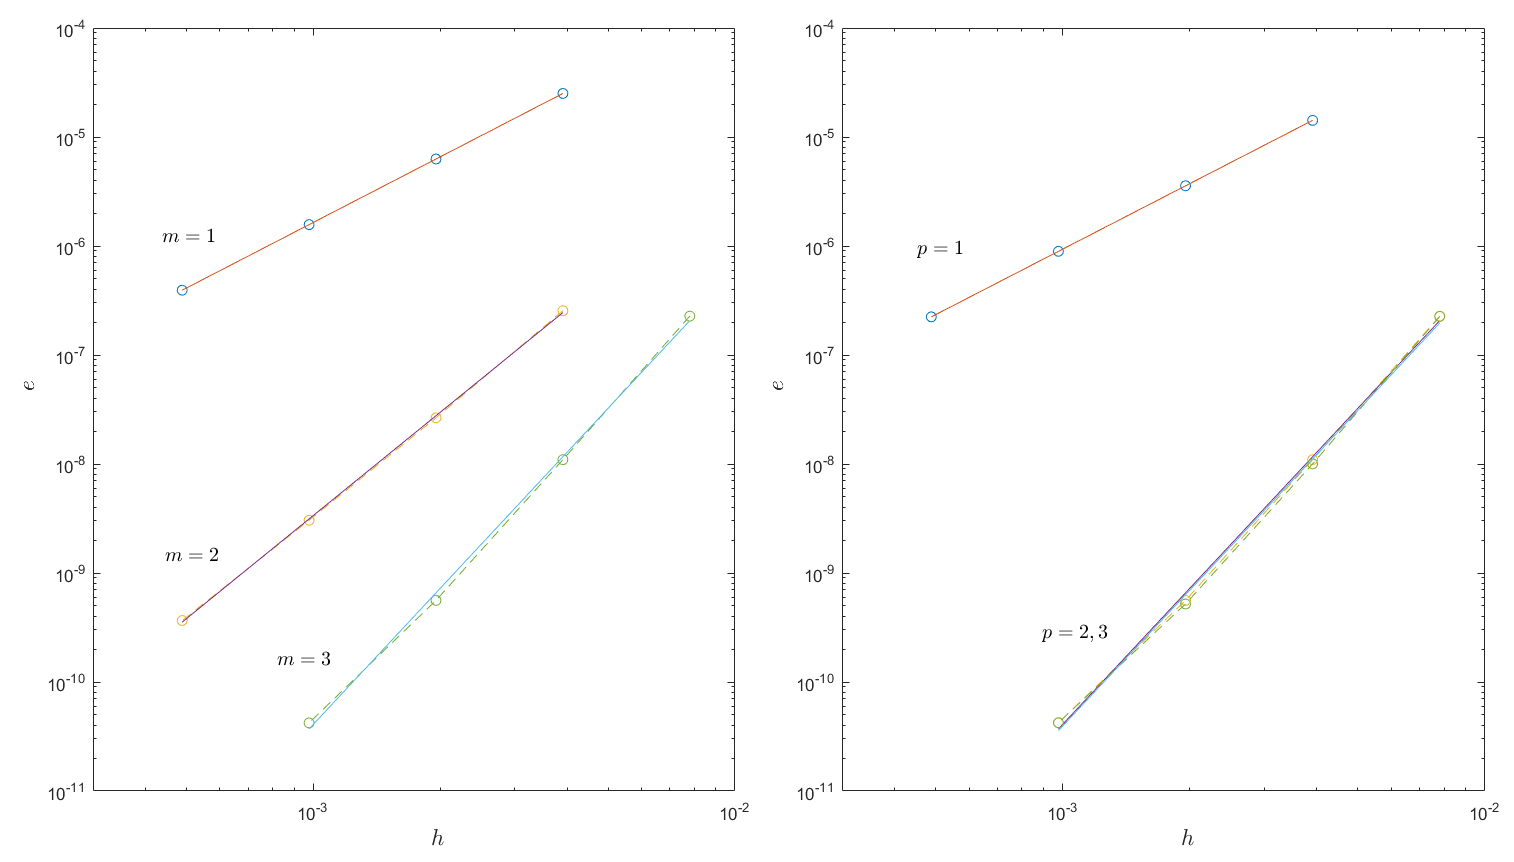
\includegraphics[width=0.95\textwidth]{Graphics/lldp-fj/mp_new.png}}
	\caption{Gráfico Log-log de error ${e_i=\max_{t_n\in(t)_{h_i}}\nnnorm{y_n-x(t_n)}_\infty}$ contra $h_i$ integrando la ecuación de Ejemplo \ref{ex:Brus} con el esquema (\ref{JFLLRK4}), fijados $\eta_1=\eta_2=2$, $\alpha_1=\alpha_2=0.5$, $\beta=1$ y $h_i=2^{-i}$, $i=7,8,9,10,11$, y : Izquierda, $\mf=1,2,3$, $\pf=2$; y Derecha, $\pf=1,2,3$, $\mf=3$.} \label{Fig1}
\end{figure}

\begin{table}[htb]
	\centering
	\caption{
		Orden de convergencia $r$ del esquema (\ref{JFLLRK4}) y las estimaciones $\widetilde{r}$ para diferentes valores de $\mf$ y $\pf$, el $90\%$ límite de confianza $\Delta$ de $\widetilde{r}$, y el coeficiente de determinación $R^2$ de la recta ajustada en Figura \ref{Fig1}. Lo valores $\eta_1=\eta_2=2$, $\alpha_1=\alpha_2=0.5$ y $\beta=1$ se mantienen fijos.}
	\begin{adjustbox}{width=0.8\columnwidth,center}
		\begin{tabular}{cccccllccccc}
			\cline{1-12}
			&  & $\pf=2$ &  &  &  &  &  &  & $\mf=3$ &  &  \\ \cline{2-5}\cline{9-12}
			$\mf$ & $r$ & $\widetilde{r}$ & $\pm \varDelta$ & $R^{2}$ &  &  & $\pf+\pf$
			& $r$ & $\widetilde{r}$ & $\pm \varDelta$ & $R^{2}$ \\ 
			\cline{1-5}\cline{8-12}
			1 & 2 & 1.999 & 0.001 & 0.98 &  &  & 2 & 2 & 1.996 & 0.003 & 0.98 \\ 
			2 & 3 & 3.145 & 0.149 & 0.98 &  &  & 4 & 4 & 4.148 & 0.476 & 0.98 \\ 
			3 & 4 & 4.148 & 0.476 & 0.98 &  &  & 6 & 4 & 4.141 & 0.633 & 0.98 \\ 
			\cline{1-12}
		\end{tabular}
	\end{adjustbox}
	\label{tab:mporders}
\end{table}


Los errores $e_i=\max_{t_n\in(t)_{h_i}}\nnnorm{y_n-x(t_n)}_\infty$ del código \textit{JF-LLRK} en la integración de la ecuación de Brusselator fueron calculados para diferentes discretizaciones de tiempo $(t)_{h_i}$ con un tamaño de paso fijo $h_i$, donde la \textquotedblleft solución exacta\textquotedblright ~$x$ se estima mediante el código Matlab \textit{ode15s} con tolerancias $RTol= 10^{-12}$ y $ATol=10^{-14}$. La Figura \ref{Fig1}-izquierda muestra cuatro de estos errores para el código \textit{JF-LLRK} con diferentes valores de $\mf$, y fijo $\pf=2$, $\eta_1=\eta_2=2$ , $\alpha_1=\alpha_2=0.5$ y $\beta=1$, así como la recta ajustada a los puntos $(\log_2(h_i),\log_2(e_i))$ con $i=1,. ..,4$. La Tabla \ref{tab:mporders}-izquierda presenta el valor de la pendiente $\widetilde{r}$ de la línea recta ajustada para cada valor de $\mf$, lo que proporciona una estimación del orden de convergencia del esquema. La tabla también presenta los $90\%$ límites de confianza de $\widetilde{r}$, el coeficiente de determinación como indicador de la bondad de la línea ajustada, y el orden de convergencia de convergencia esperado $r$ que - de acuerdo con el Teorema \ref {theorem:kp-fj-llrk-convergence} - el esquema (\ref{JFLLRK4}) tiene para los diferentes valores de $\mf$. La Figura \ref{Fig1}-derecha y la Tabla \ref{tab:mporders}-derecha presentan resultados similares pero para el código \textit{JF-LLRK} con varios valores de $\pf$ y $\mf=3$ fijados $\eta_1=\eta_2=2$, $\alpha_1=\alpha_2=0.5$ y $\beta=1$. Observe que el orden de convergencia de convergencia estimado $\widetilde{r}$ proporcionado en la Tabla \ref{tab:mporders} está de acuerdo con el orden de convergencia del esquema (\ref{JFLLRK4}) establecido por el Teorema \ref{theorem:kp-fj-llrk-convergence} para los valores considerados de $\mf$ y $\pf$.

Análogamente, las Figuras \ref{Fig2}, \ref{Fig3} y las Tablas \ref{tab:out}, \ref{tab:in} presentan los resultados de las simulaciones correspondientes al orden de de convergencia del esquema (\ref{JFLLRK4}) en función de los parámetros de sus dos aproximaciones libres de Jacobiano. Nuevamente el orden de convergencia de convergencia estimado $\widetilde{r}$ proporcionado en las Tablas \ref{tab:in} y \ref{tab:out} está de acuerdo con el orden de convergencia de convergencia del esquema (\ref{JFLLRK4}) establecido por Teorema \ref{theorem:kp-fj-llrk-convergence} para los valores considerados de $\eta_1$, $\eta_2$, $\alpha_1$, $\alpha_2$ y $\beta$.


\begin{figure}[htb]
	\centering
	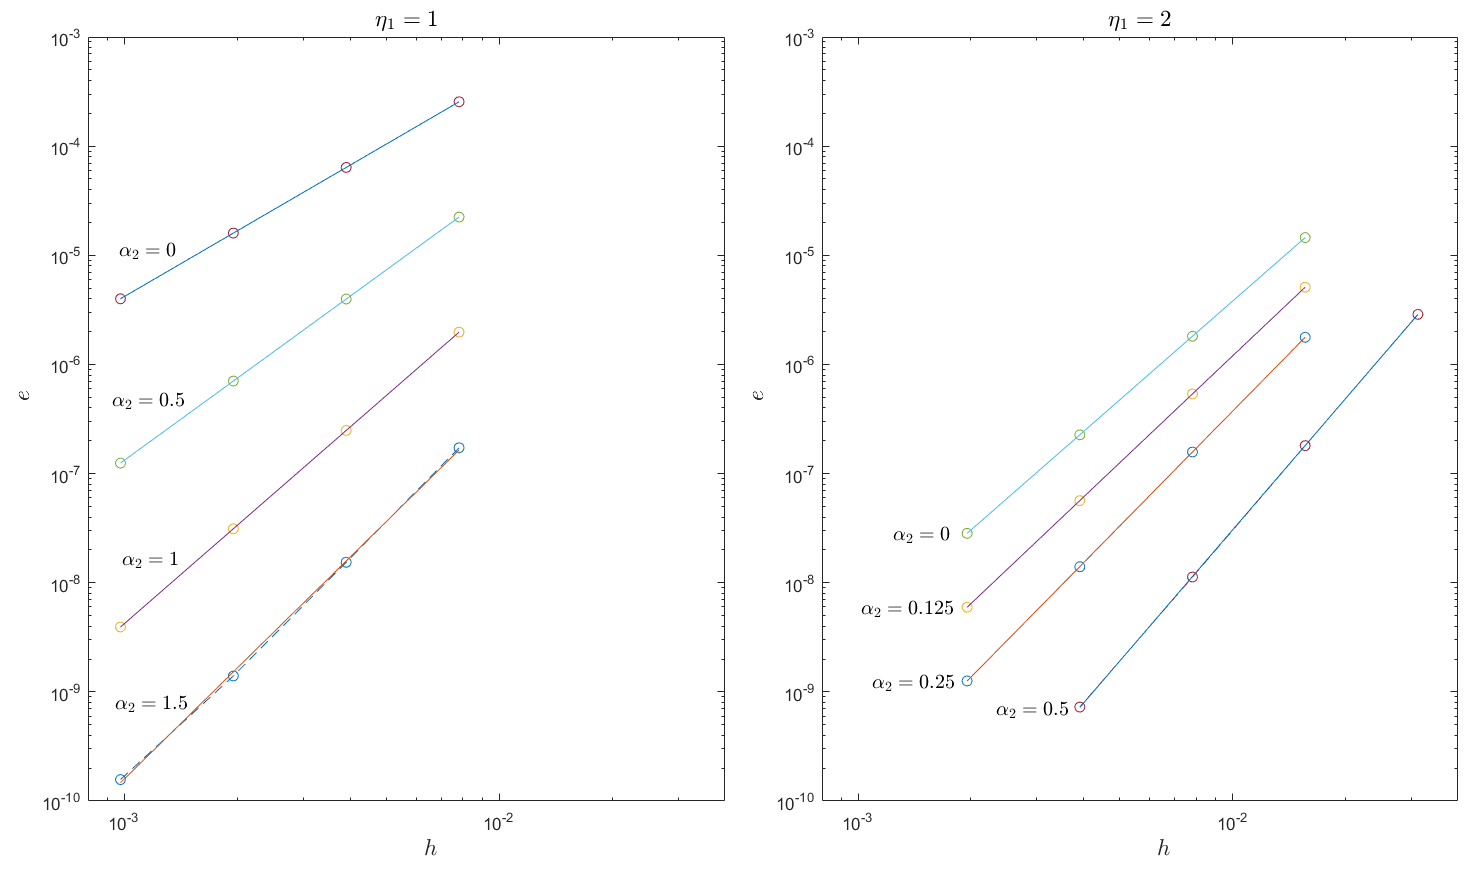
\includegraphics[width=0.95\textwidth]{Graphics/lldp-fj/out_new.png}
	\caption{Gráfico Log-log de error $e_i=\max_{t_n\in(t)_{h_i}}\nnnorm{y_n-x(t_n)}_\infty$ contra $h_i$ integrando la ecuación de Ejemplo \ref{ex:Brus} con el esquema (\ref{JFLLRK4}), fijados $\mf=14$, $\pf=4$, $\eta_1=2$, $\alpha_1=0.5$, $\beta=1$, y: Izquierda, $\eta_2=1$, $\alpha_2=0,0.5,1,1.5$, $h_i=2^{-i}$, $i=7,8,9,10$ y Derecha, $\eta_2=2$, $\alpha_2=0,0.125,0.25,0.5$, $h_i=2^{-i}$, $i=5,6,7,8,9$.}
	\label{Fig2}
\end{figure}

\begin{table}[htb]
	\centering
	\caption{
		Orden de convergencia $r$ del esquema (\ref{JFLLRK4}) y las estimaciones $\widetilde{r}$ para diferentes valores de $\eta_2$ y $\alpha_2$, el $90\%$ límite de confianza $\Delta$ de $\widetilde{r}$, el coeficiente de determinación $R^2$ de la recta ajustada en Figura \ref{Fig2}. Los valores de $\mf=14$, $\pf=4$, $\eta_1=2$, $\alpha_1=0.5$ y $\beta=1$ se mantienen fijos. }
	\begin{adjustbox}{width=0.8\columnwidth,center}
		\begin{tabular}{ c  c c c c  c  c c c c c}
			\hline
			& \multicolumn{4}{c}{$\eta_2=1$} & & & \multicolumn{4}{c}{$\eta_2=2$} \\
			\cline{2-5} \cline{8-11}
			$\alpha_2$ & $r$ & $\widetilde{r}$ & $\pm\varDelta$ & $R^2$ & & $\alpha_2$ & $r$ & $\widetilde{r}$ & $\pm\varDelta$ & $R^2$ \\
			\hline
			0 & 2 & 1.999 & 0.001 & 0.98 & & 0 & 3 & 3.000 & 0.002 & 0.97 \\
			0.5 & 2.5 & 2.496 & 0.003 & 0.98 & & 0.125 & 3.25 & 3.247 & 0.003 & 0.97 \\
			1 & 3 & 2.992 & 0.005 & 0.98 & & 0.25 & 3.5 & 3.487 & 0.013 & 0.97 \\
			1.5 & 3.5 & 3.376 & 0.025 & 0.98 & & 0.5 & 4 & 3.986 & 0.029 & 0.97 \\
			\hline
		\end{tabular}
	\end{adjustbox}
	\label{tab:out}
\end{table}


\begin{figure}[htb]
	\centering
	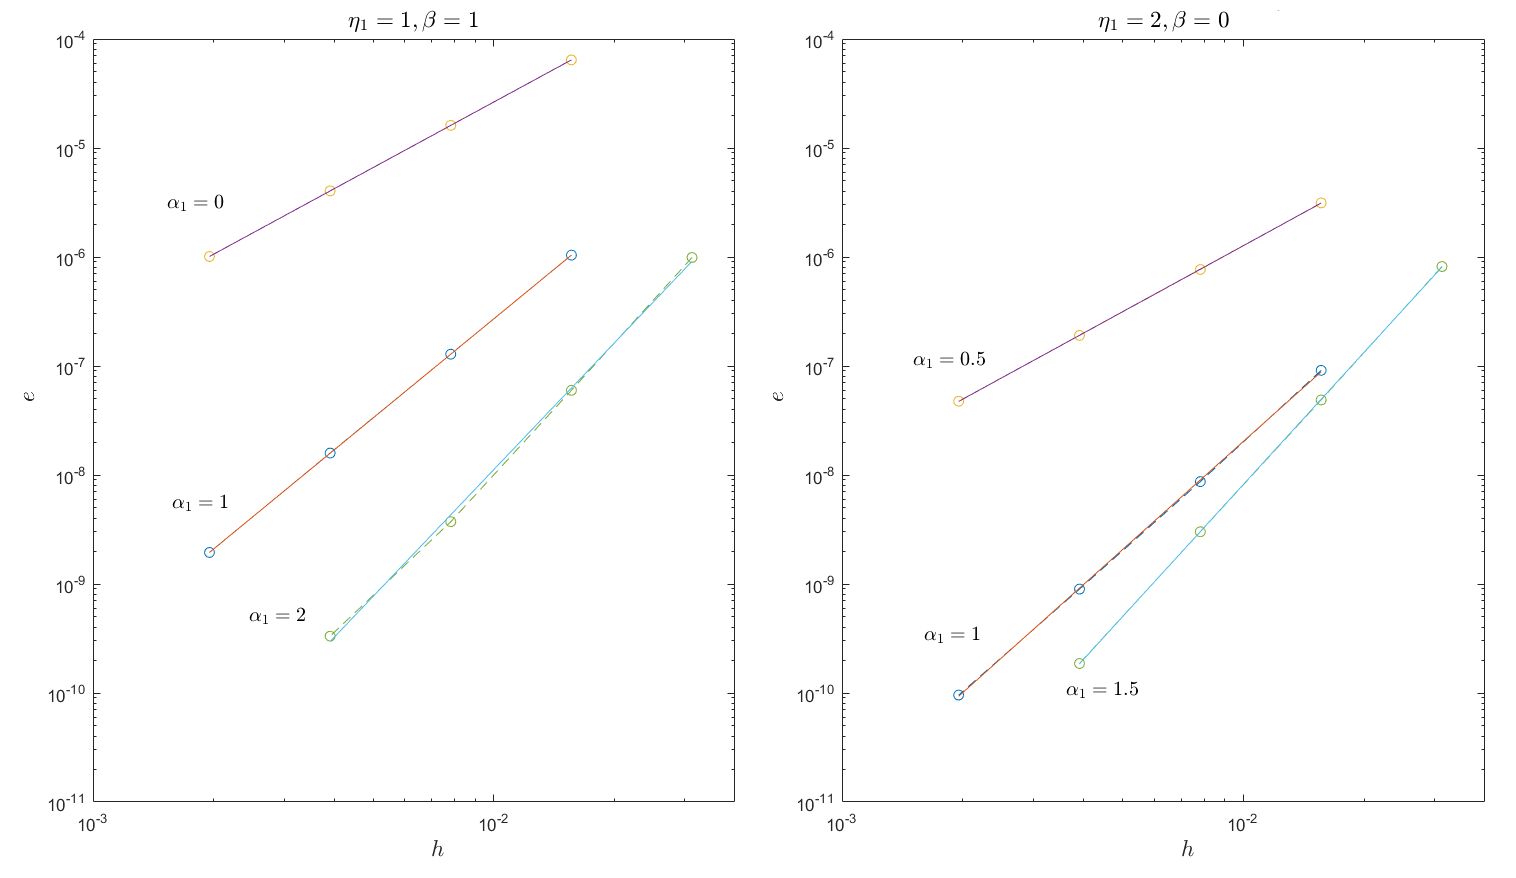
\includegraphics[width=0.95\textwidth]{Graphics/lldp-fj/in_new.png}
	\caption{Gráfico Log-log de error $e_i=\max_{t_n\in(t)_{h_i}}\nnnorm{y_n-x(t_n)}_\infty$ contra $h_i$ integrando la ecuación de Ejemplo \ref{ex:Brus} con el esquema (\ref{JFLLRK4}), fijados $\mf=14$, $\pf=4$, $\eta_2=2$, $\alpha_2=1$, $h_i=2^{-i}$, $i=5,6,7,8,9$, y: Izquierda, $\alpha_1=0,1,2$ para $\eta_1=1,\beta=1$; Derecha, $\alpha_1=0.5,1,1.5$ para $\eta_1=2,\beta=0$.}
	\label{Fig3}
\end{figure}


\begin{table}[htb]
	\centering
	\caption{
        Orden de convergencia $r$ del esquema (\ref{JFLLRK4}) y las estimaciones $\widetilde{r}$ para diferentes valores de  $\eta_1$, $\alpha_1$ y $\beta$, el $90\%$ límite de confianza $\Delta$ de $\widetilde{r}$, el coeficiente de determinación $R^2$ de la recta ajustada en Figura \ref{Fig3}. Los valores de $\mf=14$, $\pf=4$, $\eta_2=2$ y$\alpha_2=1$ se mantienen fijos.}
	\begin{adjustbox}{width=0.8\columnwidth,center}
		\begin{tabular}{ccccccccccccc}
			\hline
			&  & \multicolumn{4}{c}{$\eta _{1}=1$} &  &  &  & \multicolumn{4}{c}{$\eta
				_{1}=2$} \\ \cline{3-6}\cline{10-13}
			$\beta $ & $\alpha _{1}$ & $r$ & $\widetilde{r}$ & $\pm \varDelta$ & $R^{2}$
			&  & $\beta $ & $\alpha _{1}$ & $r$ & $\widetilde{r}$ & $\pm \varDelta$ & $%
			R^{2}$ \\ \hline
			1 & 0 & 2 & 1.997 & 0.004 & 0.97 &  & 0 & 0.5 & 2 & 2.014 & 0.017 & 0.97 \\ 
			1 & 1 & 3 & 3.020 & 0.010 & 0.97 &  & 0 & 1 & 3 & 3.300 & 0.116 & 0.97 \\ 
			1 & 2 & 4 & 3.863 & 0.421 & 0.97 &  & 0 & 1.5 & 4 & 4.031 & 0.039 & 0.97 \\ 
			\hline
		\end{tabular}
	\end{adjustbox}
	\label{tab:in}
\end{table}

\subsubsection{Simulaciones comparativas}\label{sc:comparison}

En este conjunto de simulaciones, se utilizaran los PVI resultantes de la discretización espacial de cuatro EDP empleadas con frecuencia en la literatura. Estas ecuaciones son: Brusselator 2D (Ejemplo \ref{ex:Brus}), Brusselator 2D (Ejemplo \ref{ex:Brus2D}), Burger's (Ejemplo \ref{ex:Burger}) y Gray-Scott 2D~(Ejemplo \ref{ex:GS2D}).

Para cada ecuación de prueba, los resultados de la integración numérica se sintetizan en los diagramas de tiempo-precisión de la Figura \ref{work-precision diagram}. En estos diagramas, la precisión de los códigos \textit{JF-LLRK4}, \textit{JF-Exp4}, \textit{JF-EPIRK4} y \textit{BDF4} se mide por el error $e_i=\max\limits_ {t_n\in(t)_{h_i}}\nnnorm{y_n-x(t_n)}_\infty$ entre la \textquotedblleft solución exacta\textquotedblright~$x$ de la ecuación de prueba y la solución aproximada $y_n$ de cada código calculado en cinco particiones de tiempo con un tamaño de paso fijo $h_i$, donde la \textquotedblleft solución exacta\textquotedblright ~$x $ se estima nuevamente como en las simulaciones preliminares. La Figura \ref{work-precision diagram} muestra que, para estas ecuaciones, el esquema LLRK libre de Jacobiano (\ref{JFLLRK4}) exhibe una precisión similar o mayor que los otros tres integradores libres de Jacobiano, pero con un costo computacional menor o similar. Esta diferencia en el tiempo computacional se explica por los resultados de las Tablas \ref{tab:br}-\ref{tab:gs2d}.

\begin{figure}[htb]
	\centering
	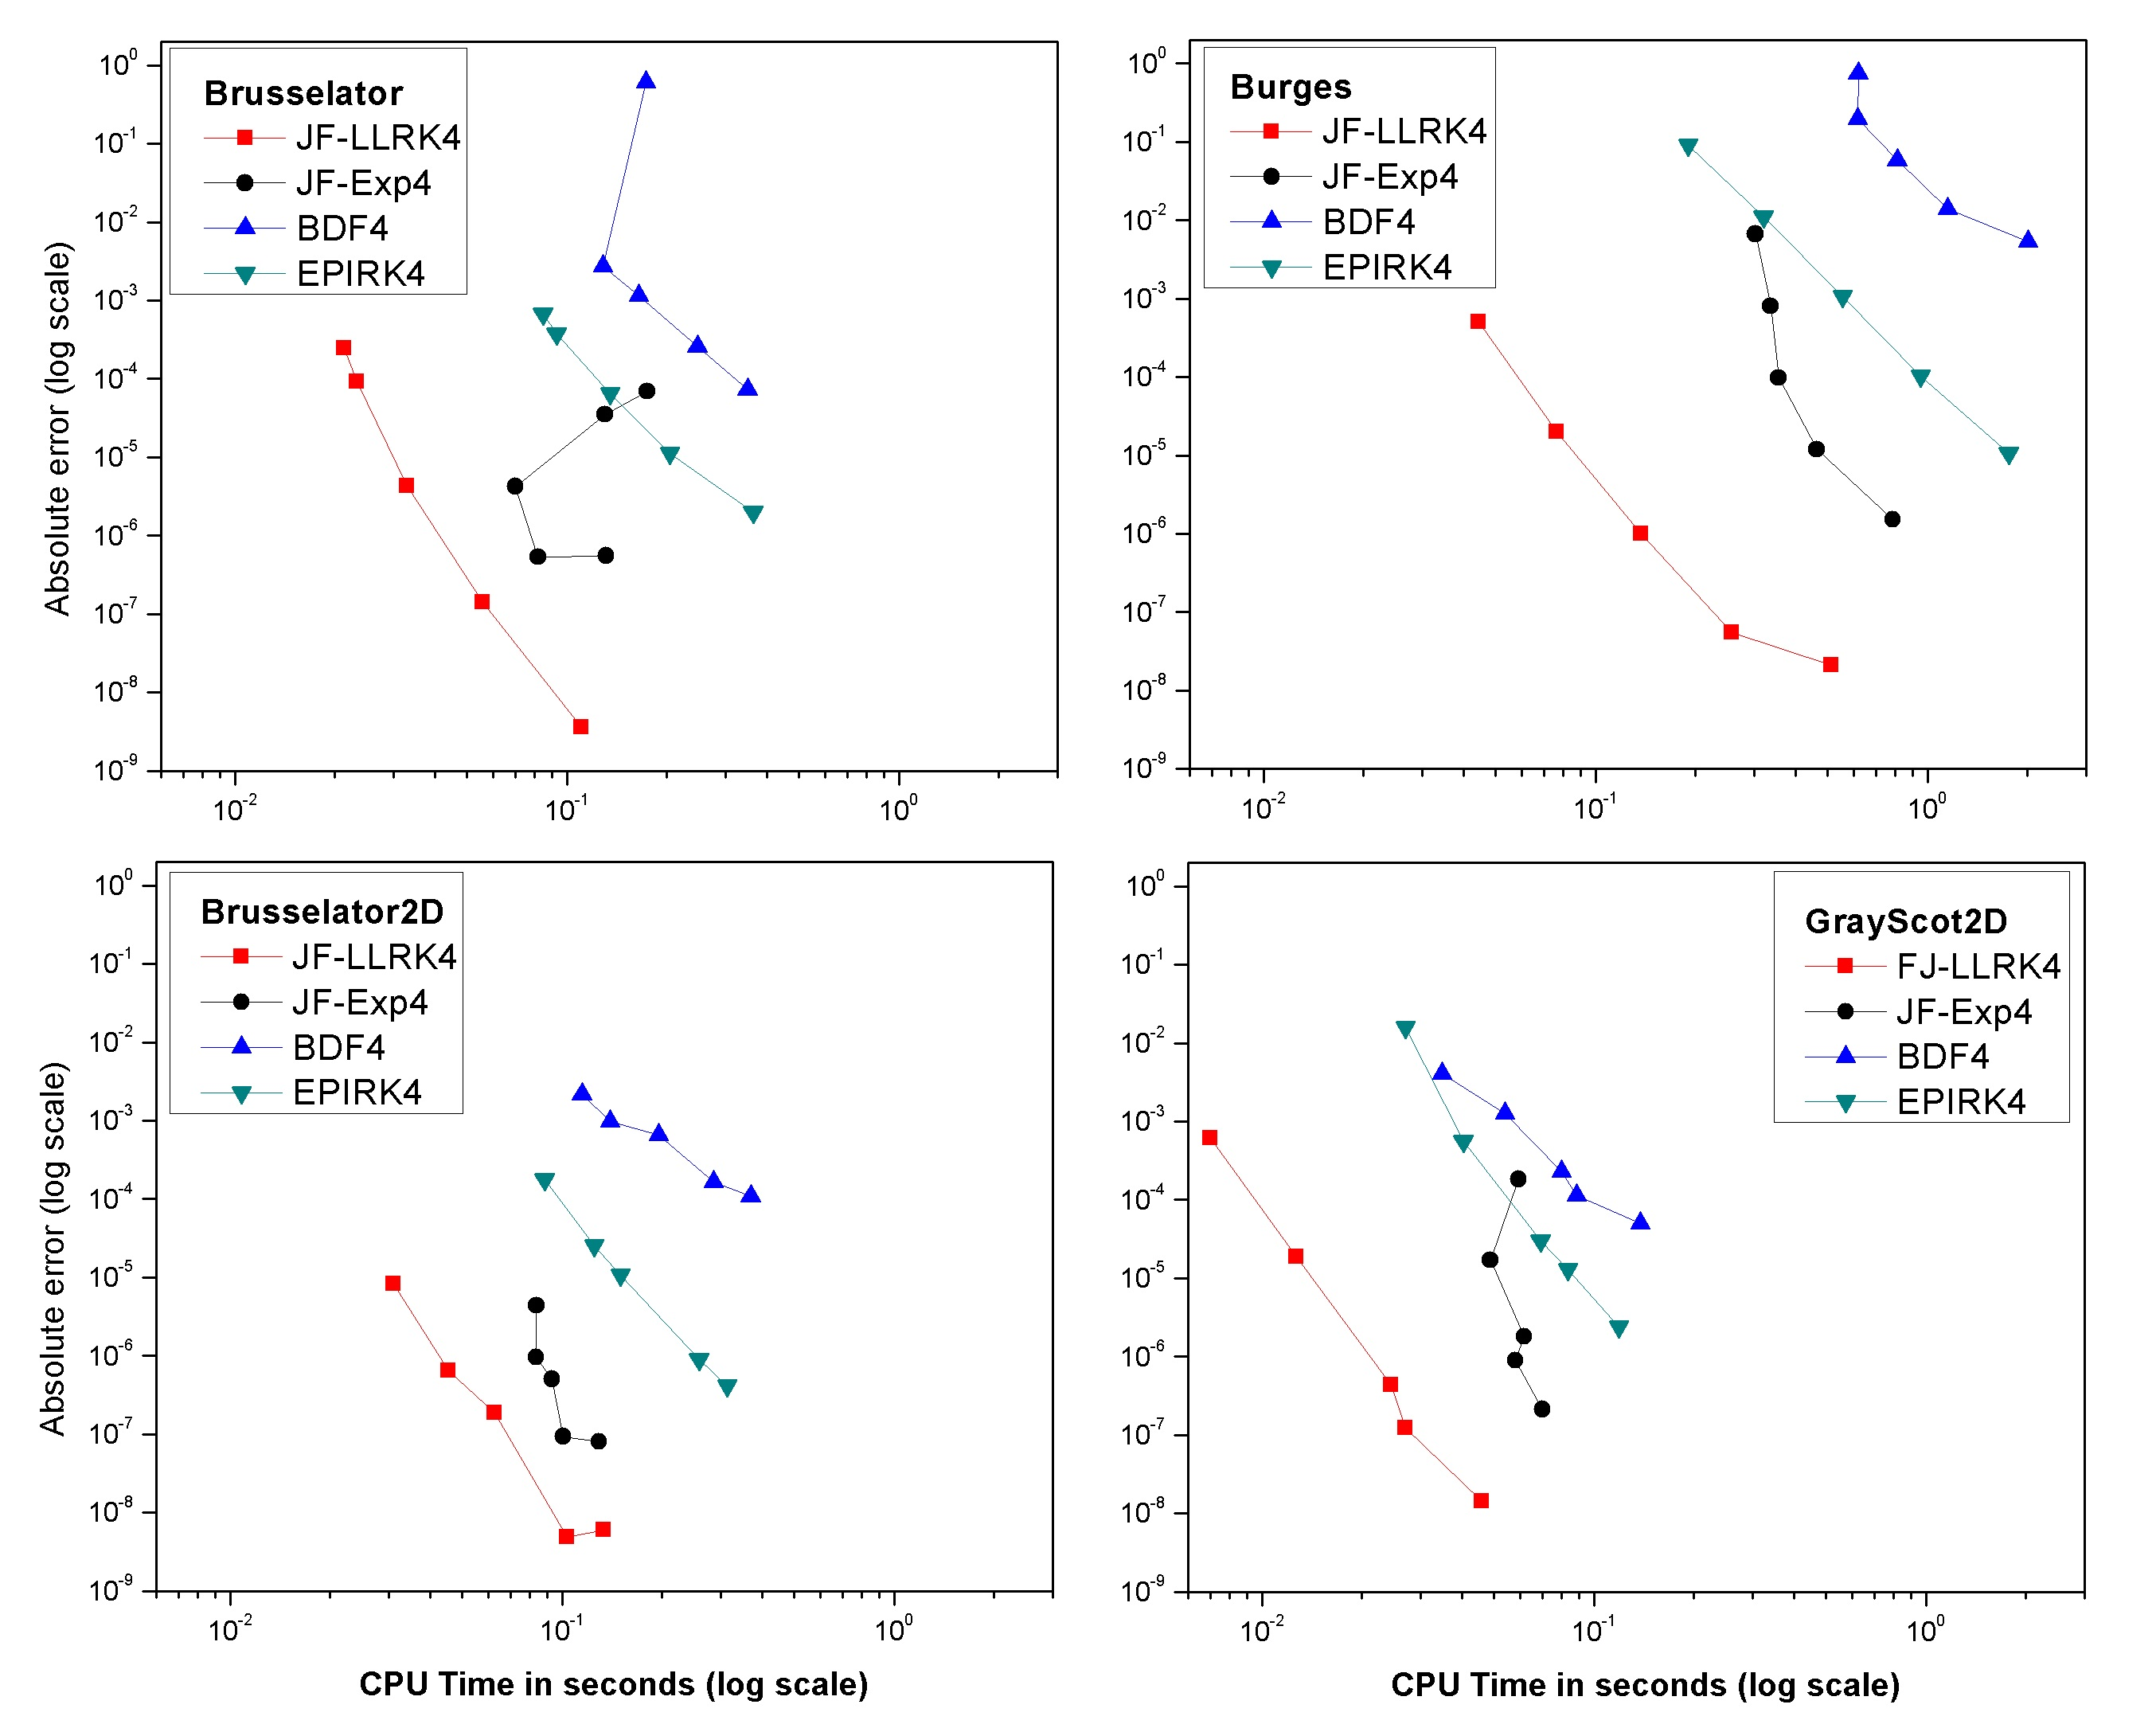
\includegraphics[width=1\textwidth]{Graphics/lldp-fj/Diagram_new.jpg}
	\caption{Diagramas comparativos de precisión contra tiempo en escala log-log para cada uno de los cuatro códigos en la integración delas cuatro ecuaciones de prueba.} \label{work-precision diagram}
\end{figure}

Para cada código, las Tablas \ref{tab:br}-\ref{tab:gs2d} presentan el tamaño del paso \textit{h}, el número de pasos \textit{Pasos}, el número de evaluaciones del campo vectorial \textit{f-Eval}, el número de aproximaciones del subespacio Krylov \textit{K-subspace} a los productos de la función phi por un vector, el número de sistemas lineales en el código \textit{BDF4} resuelto por el método General Minimal Residue \textit {GMRES}, y el número de aproximaciones de Padé \textit{Padé} requeridas por los tres integradores exponenciales. Además, la dimensión mínima $\mf_{min}$, máxima $\mf_{max}$ y total $\mf_{total}$ de los subespacios de Krylov requerida por los códigos \textit{JF-LLRK4}, \textit{JF -Exp4} y \textit{JF-EPIRK4} para integrar las ecuaciones de prueba en todo el intervalo de integración también se especifica. Para el código \emph{BDF4}, $\mf_{min}$, $\mf_{max}$ y $\mf_{total}$ representan el número mínimo, máximo y total de iteraciones realizadas por el método GMRES sobre todo el intervalo de integración.

En cada paso de integración, al igual que para el esquema (5.8) de \cite{hochbruck1998exponential}, el código \textit{JF-Exp4} realiza tres descomposiciones en subespacios de Krylov y, al menos, tres aproximaciones (6,6)-Padé a la función $\varphi_1$ de las matrices de Hessenberg resultantes del Algoritmo de Arnoldi libre de Jacobiano \ref{alg:iArnoldi}. \textit{JF-Exp4} utiliza la diferencia hacia adelante directa de primer orden como una aproximación del producto de la matriz Jacobiana por un vector en el Algoritmo \ref{alg:iArnoldi}, lo cual reduce a tres el orden de convergencia del esquema (5.8) de \cite{hochbruck1998exponential} (ver Teorema 5.1 en \cite{hochbruck1998exponential}). Para estimar la dimensión de Krylov $\mf$, el código \textit{JF-Exp4} usa el algoritmo adaptativo de \cite{hochbruck1998exponential} y no hay restricción al valor mínimo para $\mf$.

El código \textit{JF-EPIRK4} requiere de las mismas descomposiciones de Krylov y un número similar de aproximaciones de Padé que el código \textit{JF-Exp4} en cada paso de integración, pero la dimensión de Krylov $\mf$ se estima automáticamente mediante el estrategia adaptativa de \cite{niesen2012algorithm} implementada en el código de Matlab \textit{phipm}.

Para resolver los sistemas algebraicos no lineales, en cada paso de integración, el código \textit{BDF4} emplea el método clásico de Newton junto con el método General Minimal Residue (GMRES) (función de Matlab \textit{gmres} con tolerancia $RTol=10^{-6}$) y la diferencia finita hacia adelante de primer orden como una aproximación al producto de la matriz Jacobiana por vector. En la función de Matlab \textit{gmres}, se eliminaron las comprobaciones computacionalmente costosas de las funciones de Matlab \textit{iterchk} y \textit{iterapp}.

\begin{table}[htb]
	\caption{Desempeño de los códigos en la integración de la ecuación Brusselator con $M=100$, $d=200$.}
	\centering
	\begin{adjustbox}{width=0.9\columnwidth,center}
		\begin{tabular}{cccccccccc}
			\hline
			\textit{h} & Código & Pasos & f-Eval & K-subspace & GMRES & Padé & $\mf_{total}$ & $\mf%
			_{min}$ & $\mf_{max}$ \\ \hline
			\multicolumn{1}{l}{0.0250} & \multicolumn{1}{l}{JF-LLRK4} & 40 & 852 & 40 &
			0 & 40 & 492 & 4 & 16 \\
			\multicolumn{1}{l}{} & \multicolumn{1}{l}{JF-Exp4} & 40 & 3324 & 120 & 0 &
			1168 & 3124 & 4 & 48 \\
			\multicolumn{1}{l}{} & \multicolumn{1}{l}{BDF4} & 40 & 7318 & 0 & 400 & 0 &
			3305 & 3 & 24 \\
			\multicolumn{1}{l}{} & \multicolumn{1}{l}{JF-EPIRK4} & 40 & 1238 & 120 & 0 &
			625 & 718 & 4 & 11 \\
			\multicolumn{1}{l}{0.0200} & \multicolumn{1}{l}{JF-LLRK4} & 50 & 967 & 50 &
			0 & 50 & 517 & 4 & 13 \\
			\multicolumn{1}{l}{} & \multicolumn{1}{l}{JF-Exp4} & 50 & 2855 & 150 & 0 &
			1147 & 2605 & 4 & 48 \\
			\multicolumn{1}{l}{} & \multicolumn{1}{l}{BDF4} & 50 & 7156 & 0 & 448 & 0 &
			2780 & 2 & 23 \\
			\multicolumn{1}{l}{} & \multicolumn{1}{l}{JF-EPIRK4} & 50 & 1425 & 150 & 0 &
			716 & 775 & 3 & 10 \\
			\multicolumn{1}{l}{0.0100} & \multicolumn{1}{l}{JF-LLRK4} & 100 & 1477 & 100
			& 0 & 100 & 577 & 4 & 10 \\
			\multicolumn{1}{l}{} & \multicolumn{1}{l}{JF-Exp4} & 100 & 1773 & 300 & 0 &
			970 & 1273 & 2 & 36 \\
			\multicolumn{1}{l}{} & \multicolumn{1}{l}{BDF4} & 100 & 6574 & 0 & 476 & 0 &
			2269 & 2 & 13 \\
			\multicolumn{1}{l}{} & \multicolumn{1}{l}{JF-EPIRK4} & 100 & 2278 & 300 & 0 &
			976 & 978 & 2 & 7 \\
			\multicolumn{1}{l}{0.0050} & \multicolumn{1}{l}{JF-LLRK4} & 200 & 2609 & 200
			& 0 & 200 & 809 & 4 & 6 \\
			\multicolumn{1}{l}{} & \multicolumn{1}{l}{JF-Exp4} & 200 & 2256 & 600 & 0 &
			1242 & 1256 & 1 & 15 \\
			\multicolumn{1}{l}{} & \multicolumn{1}{l}{BDF4} & 200 & 7055 & 0 & 588 & 0 &
			2678 & 1 & 12 \\
			\multicolumn{1}{l}{} & \multicolumn{1}{l}{JF-EPIRK4} & 200 & 3894 & 600 & 0 &
			1294 & 1294 & 1 & 5 \\
			\multicolumn{1}{l}{0.0025} & \multicolumn{1}{l}{JF-LLRK4} & 400 & 5201 & 400
			& 0 & 400 & 1601 & 4 & 5 \\
			\multicolumn{1}{l}{} & \multicolumn{1}{l}{JF-Exp4} & 400 & 3945 & 1200 & 0 &
			1945 & 1945 & 1 & 4 \\
			\multicolumn{1}{l}{} & \multicolumn{1}{l}{BDF4} & 400 & 9530 & 0 & 919 & 0 &
			3556 & 1 & 10 \\
			\multicolumn{1}{l}{} & \multicolumn{1}{l}{JF-EPIRK4} & 400 & 7287 & 1200 & 0 &
			2087 & 2087 & 1 & 3 \\
			\hline
		\end{tabular}
	\end{adjustbox}
	\label{tab:br}
\end{table}



\begin{table}[htb]
	\caption{Desempeño de los códigos en la integración de la ecuación Brusselator 2D con $M=40$, $d=3200$.}
	\centering
	\begin{adjustbox}{width=0.9\columnwidth,center}
		\begin{tabular}{cccccccccc}
			\hline
			\textit{h} & Código & Pasos & f-Eval & K-subspace & GMRES & Padé & $\mf_{total}$ & $\mf%
			_{min}$ & $\mf_{max}$ \\ \hline
			\multicolumn{1}{l}{0.01000} & \multicolumn{1}{l}{JF-LLRK4} & 10 & 144 & 10
			& 0 & 10 & 54 & 4 & 8 \\
			\multicolumn{1}{l}{} & \multicolumn{1}{l}{JF-Exp4} & 10 & 251 & 30 & 0 & 139
			& 201 & 2 & 20 \\
			\multicolumn{1}{l}{} & \multicolumn{1}{l}{BDF4} & 10 & 1243 & 0 & 86 & 0 &
			283 & 2 & 8 \\
			\multicolumn{1}{l}{} & \multicolumn{1}{l}{JF-EPIRK4} & 10 & 263 & 30 & 0 &
			129 & 133 & 3 & 6 \\
			\multicolumn{1}{l}{0.00625} & \multicolumn{1}{l}{JF-LLRK4} & 16 & 218 & 16
			& 0 & 16 & 74 & 4 & 6 \\
			\multicolumn{1}{l}{} & \multicolumn{1}{l}{JF-Exp4} & 16 & 284 & 48 & 0 & 167
			& 204 & 2 & 15 \\
			\multicolumn{1}{l}{} & \multicolumn{1}{l}{BDF4} & 16 & 1618 & 0 & 118 & 0 &
			334 & 1 & 7 \\
			\multicolumn{1}{l}{} & \multicolumn{1}{l}{JF-EPIRK4} & 16 & 383 & 48 & 0 &
			174 & 175 & 2 & 6 \\
			\multicolumn{1}{l}{0.00500} & \multicolumn{1}{l}{JF-LLRK4} & 20 & 268 & 20 &
			0 & 20 & 88 & 4 & 6 \\
			\multicolumn{1}{l}{} & \multicolumn{1}{l}{JF-Exp4} & 20 & 307 & 60 & 0 & 184
			& 207 & 2 & 15 \\
			\multicolumn{1}{l}{} & \multicolumn{1}{l}{BDF4} & 20 & 1449 & 0 & 109 & 0 &
			313 & 1 & 6 \\
			\multicolumn{1}{l}{} & \multicolumn{1}{l}{JF-EPIRK4} & 20 & 464 & 60 & 0 &
			204 & 204 & 2 & 5 \\
			\multicolumn{1}{l}{0.00250} & \multicolumn{1}{l}{JF-LLRK4} & 40 & 521 & 40 &
			0 & 40 & 161 & 4 & 5 \\
			\multicolumn{1}{l}{} & \multicolumn{1}{l}{JF-Exp4} & 40 & 455 & 120 & 0 & 251
			& 255 & 1 & 8 \\
			\multicolumn{1}{l}{} & \multicolumn{1}{l}{BDF4} & 40 & 1452 & 0 & 120 & 0 &
			384 & 1 & 5 \\
			\multicolumn{1}{l}{} & \multicolumn{1}{l}{JF-EPIRK4} & 40 & 846 & 120 & 0 &
			326 & 326 & 1 & 4 \\
			\multicolumn{1}{l}{0.00200} & \multicolumn{1}{l}{JF-LLRK4} & 50 & 650 & 50
			& 0 & 50 & 200 & 4 & 4 \\
			\multicolumn{1}{l}{} & \multicolumn{1}{l}{JF-Exp4} & 50 & 541 & 150 & 0 & 289
			& 291 & 1 & 8 \\
			\multicolumn{1}{l}{} & \multicolumn{1}{l}{BDF4} & 50 & 1785 & 0 & 150 & 0 &
			457 & 1 & 5 \\
			\multicolumn{1}{l}{} & \multicolumn{1}{l}{JF-EPIRK4} & 50 & 1027 & 150 & 0 &
			377 & 377 & 1 & 4 \\
			\hline
		\end{tabular}
	\end{adjustbox}
	\label{tab:br2d}
\end{table}

\begin{table}[htb]
	\caption{Desempeño de los códigos en la integración de la ecuación Burger's con $M=400$, $d=400$.}
	\centering
	\begin{adjustbox}{width=0.9\columnwidth,center}
		\begin{tabular}{cccccccccc}
			\hline
			\textit{h} & Código & Pasos & f-Eval & K-subspace & GMRES & Padé & $\mf_{total}$ & $\mf%
			_{min}$ & $\mf_{max}$ \\ \hline
			\multicolumn{1}{l}{0.0050000} & \multicolumn{1}{l}{JF-LLRK4} & 100 & 1614 &
			100 & 0 & 100 & 714 & 4 & 10 \\
			\multicolumn{1}{l}{} & \multicolumn{1}{l}{JF-Exp4} & 100 & 6104 & 300 & 0 &
			2507 & 5604 & 3 & 27 \\
			\multicolumn{1}{l}{} & \multicolumn{1}{l}{BDF4} & 100 & 17304 & 0 & 910 & 0
			& 6469 & 2 & 12 \\
			\multicolumn{1}{l}{} & \multicolumn{1}{l}{JF-EPIRK4} & 100 & 2874 & 300 & 0 &
			1435 & 1574 & 3 & 7 \\
			\multicolumn{1}{l}{0.0025000} & \multicolumn{1}{l}{JF-LLRK4} & 200 & 2922 &
			200 & 0 & 200 & 1122 & 4 & 8 \\
			\multicolumn{1}{l}{} & \multicolumn{1}{l}{JF-Exp4} & 200 & 7287 & 600 & 0 &
			3784 & 6287 & 2 & 20 \\
			\multicolumn{1}{l}{} & \multicolumn{1}{l}{BDF4} & 200 & 27333 & 0 & 1665 & 0
			& 7783 & 2 & 10 \\
			\multicolumn{1}{l}{} & \multicolumn{1}{l}{JF-EPIRK4} & 200 & 4988 & 600 & 0 &
			2388 & 2388 & 2 & 5 \\
			\multicolumn{1}{l}{0.0012500} & \multicolumn{1}{l}{JF-LLRK4} & 400 & 5361 &
			400 & 0 & 400 & 1761 & 4 & 5 \\
			\multicolumn{1}{l}{} & \multicolumn{1}{l}{JF-Exp4} & 400 & 8123 & 1200 & 0 &
			4975 & 6123 & 1 & 11 \\
			\multicolumn{1}{l}{} & \multicolumn{1}{l}{BDF4} & 400 & 37402 & 0 & 2454 & 0
			& 9416 & 2 & 10 \\
			\multicolumn{1}{l}{} & \multicolumn{1}{l}{JF-EPIRK4} & 400 & 9111 & 1200 & 0 &
			3911 & 3911 & 1 & 4 \\
			\multicolumn{1}{l}{0.0006250} & \multicolumn{1}{l}{JF-LLRK4} & 800 & 10400 &
			800 & 0 & 800 & 3200 & 4 & 4 \\
			\multicolumn{1}{l}{} & \multicolumn{1}{l}{JF-Exp4} & 800 & 11223 & 2400 & 0
			& 7039 & 7223 & 1 & 8 \\
			\multicolumn{1}{l}{} & \multicolumn{1}{l}{BDF4} & 800 & 32269 & 0 & 2251 & 0
			& 8838 & 2 & 5 \\
			\multicolumn{1}{l}{} & \multicolumn{1}{l}{JF-EPIRK4} & 800 & 16766 & 2400 & 0 &
			6366 & 6366 & 1 & 4 \\
			\multicolumn{1}{l}{0.0003125} & \multicolumn{1}{l}{JF-LLRK4} & 1600 & 20800
			& 1600 & 0 & 1600 & 6400 & 4 & 4 \\
			\multicolumn{1}{l}{} & \multicolumn{1}{l}{JF-Exp4} & 1600 & 19555 & 4800 & 0
			& 11555 & 11555 & 1 & 4 \\
			\multicolumn{1}{l}{} & \multicolumn{1}{l}{BDF4} & 1600 & 58643 & 0 & 4360 & 0
			& 17910 & 2 & 8 \\
			\multicolumn{1}{l}{} & \multicolumn{1}{l}{JF-EPIRK4} & 1600 & 31872 & 4800 & 0 &
			11072 & 11072 & 1 & 3 \\
			\hline
		\end{tabular}
	\end{adjustbox}
	\label{tab:bg}
\end{table}


\begin{table}[htb]
	\caption{Desempeño de los códigos en la integración de la ecuación Gray-Scott 2D con $M=20$, $d=800$.}
	\centering
	\begin{adjustbox}{width=0.9\columnwidth,center}
		\begin{tabular}{cccccccccc}
			\hline
			\textit{h} & Código & Pasos & f-Eval & K-subspace & GMRES & Padé & $\mf_{total}$ & $\mf%
			_{min}$ & $\mf_{max}$ \\ \hline
			0.010000 & \multicolumn{1}{l}{JF-LLRK4} & 10 & 161 & 10 & 0 & 10 & 71 & 4 &
			10 \\
			& \multicolumn{1}{l}{JF-Exp4} & 10 & 656 & 30 & 0 & 258 & 606 & 4 & 36 \\
			& \multicolumn{1}{l}{BDF4} & 10 & 923 & 0 & 52 & 0 & 332 & 2 & 14 \\
			& \multicolumn{1}{l}{JF-EPIRK4} & 10 & 296 & 30 & 0 & 148 & 166 & 4 & 9 \\
			0.005000 & \multicolumn{1}{l}{JF-LLRK4} & 20 & 296 & 20 & 0 & 20 & 116 & 4 &
			8 \\
			& \multicolumn{1}{l}{JF-Exp4} & 20 & 643 & 60 & 0 & 327 & 543 & 2 & 27 \\
			& \multicolumn{1}{l}{BDF4} & 20 & 1064 & 0 & 72 & 0 & 371 & 1 & 10 \\
			& \multicolumn{1}{l}{JF-EPIRK4} & 20 & 494 & 60 & 0 & 228 & 234 & 2 & 7 \\
			0.002500 & \multicolumn{1}{l}{JF-LLRK4} & 40 & 547 & 40 & 0 & 40 & 187 & 4 &
			8 \\
			& \multicolumn{1}{l}{JF-Exp4} & 40 & 787 & 120 & 0 & 439 & 587 & 1 & 20 \\
			& \multicolumn{1}{l}{BDF4} & 40 & 1308 & 0 & 101 & 0 & 468 & 2 & 7 \\
			& \multicolumn{1}{l}{JF-EPIRK4} & 40 & 889 & 120 & 0 & 369 & 369 & 1 & 5 \\
			0.002000 & \multicolumn{1}{l}{JF-LLRK4} & 50 & 669 & 50 & 0 & 50 & 219 & 4 &
			6 \\
			& \multicolumn{1}{l}{JF-Exp4} & 50 & 876 & 150 & 0 & 488 & 626 & 1 & 15 \\
			& \multicolumn{1}{l}{BDF4} & 50 & 1472 & 0 & 118 & 0 & 528 & 2 & 7 \\
			& \multicolumn{1}{l}{JF-EPIRK4} & 50 & 1079 & 150 & 0 & 429 & 429 & 1 & 5 \\
			0.001250 & \multicolumn{1}{l}{JF-LLRK4} & 80 & 1050 & 80 & 0 & 80 & 330 & 4
			& 6 \\
			& \multicolumn{1}{l}{JF-Exp4} & 80 & 1118 & 240 & 0 & 619 & 718 & 1 & 15 \\
			& \multicolumn{1}{l}{BDF4} & 80 & 2151 & 0 & 184 & 0 & 715 & 1 & 6 \\
			& \multicolumn{1}{l}{JF-EPIRK4} & 80 & 1626 & 240 & 0 & 586 & 586 & 1 & 4 \\
			\hline
		\end{tabular}
	\end{adjustbox}
	\label{tab:gs2d}
\end{table}


Se puede observar de las Tablas \ref{tab:br}-\ref{tab:gs2d}, que el código \textit{BDF4} requiere de un número mucho mayor de evaluaciones del campo vectorial que los otros tres códigos, lo que explica su mayor costo computacional en los diagramas tiempo-precisión de la Figura \ref{work-precision diagram}. Por otro lado, para los tamaños de paso más grandes, el número de evaluaciones del campo vectorial de los códigos \textit{JF-Exp4} y \textit{JF-EPIRK4} es mayor que el del código \textit{JF-LLRK4}, por lo que su costo computacional es mucho mayor que el del código \textit{JF-LLRK4}. Para los tamaños de paso más pequeños, el número de evaluaciones del campo vectorial del código \textit{JF-Exp4} es ligeramente inferior o similar al del código \textit{JF-LLRK4}, lo que explica el costo computacional similar de estos dos códigos en los diagramas tiempo-precisión correspondientes a las ecuaciones Brusselator y Brusselator 2D de la Figura \ref{work-precision diagram}.

Además, las Tablas \ref{tab:br}-\ref{tab:gs2d} muestran la efectividad de la estrategia del código \textit{JF-LLRK4} para la selección de la dimensión Krylov $\mf$ en cada paso de integración, con mínima variación entre los valores de $\mf_{min}$ y $\mf_{max}$, y por tanto, con un valor de $\mf_{total}$ mucho menor que los demás códigos.

En resumen, las simulaciones han demostrado que, con un costo computacional similar, el nuevo integrador libre de Jacobiano presenta una precisión mucho mayor que los otros tres integradores libres de Jacobiano; mientras que, con una precisión similar, el primero es mucho más rápido que los segundos.

Para concluir esta sección, recordemos que la selección de $\delta$ y $h$ en esquemas prácticos libres de Jacobiano se realiza bajo diferentes criterios que resultan en valores óptimos para $\delta$ y $h$ independientes entre sí \cite{knoll2004jacobian}. Con este conocimiento en mente, la teoría desarrollada hasta este punto y los experimentos numéricos realizados con $\delta$ vinculados a una potencia de $h$ pretenden sentar las bases para diseñar esquemas prácticos Localmente Linealizados de Orden Superior Libres Jacobiano con valores óptimos de $h$ y $\delta$.

\section{Esquema Runge-Kutta de Dormand y Prince Localmente Linealizado}
En ésta sección, se combinan las aproximaciones Krylov-Padé libre de Jacobiano del Capítulo \ref{chapter:solve-non-smal-lineal-eq} con las fórmulas Runge-Kutta embebidas de Dormand y Prince Localmente Linealizadas para implementar un esquema adaptativo de orden variable libre de Jacobiano.

Utilizando la aproximación $(\mf , \pf ,\qf , k)$-Krylov-Padé Libre de Jacobiano
\begin{equation}
\widetilde{u}_j=\widehat{K}_{\mf,k}^{\pf,\qf}\left(c_j h_n, f_x(y_n) , f(y_n); \eta_1, \delta_1, \beta \right) \label{eq:approx_u_j},
\end{equation}
definida en (\ref{eq:gen_kp_aprox_fj}), para las $u_j$ en las fórmulas embebidas (\ref{lldis}) y las aproximaciones libres de Jacobiano $g_2(y_n,\widetilde{u}_j;\delta_2)$ al producto  $f_x(y_n)\widetilde{u}_j$ en (\ref{lldis}), obtenemos la Fórmulas de Runge-Kutta localmente linealizadas libres de Jacobiano
\begin{equation}
	y_{n+1}\,=\,y_n+\widetilde{u}_s+h_n \sum_{j=1}^{s}b_j \widetilde{\kt}_j \,\,\, \text{y} \,\,\, \
	\widehat{y}_{n+1}\,=\, y_n+\widetilde{u}_s+h_n \sum_{j=1}^{s}\widehat{b}_j \widetilde{\kt}_j, \label{Jacobian-free LLDPK scheme}
	\end{equation}
para integrar PVI de grandes dimensiones, donde
\begin{equation*}
	\widetilde{\kt}_j = f\left( y_n+\widetilde{u}_j+h_n \sum_{i=1}^{j-1}a_{j,i}\widetilde{\kt}_i \right) - f( y_n) - g_2(y_n,\widetilde{u}_j;\delta_2),
\end{equation*}
y $\widetilde{\kt}_1=0$, son $a_{j,i}$, $b_j$, $\widehat{b}_j$ los coeficientes de Runge-Kutta de  Dormand y Prince definidos en la Tabla \ref{ButcherTabla} y  $g_2(y_n,\widetilde{u}_j;\delta_2)$ es la aproximación de $f_x(y_n)\widetilde{u}_j$ que satisface la cota~(\ref{eq:g_bound2}).

El siguiente teorema trata sobre la velocidad de convergencia de las fórmulas embebidas (\ref{Jacobian-free LLDPK scheme}). Con este propósito, estas fórmulas se reescriben como
\begin{equation*}
    y_{n+1}=y_{n}+\digamma (y_{n};h_{n})\text{ \ \ \ \ y \ \ \ \ }\widehat{y}_{n+1}=y_{n}+\widehat{\digamma }(y_{n};h_{n}).
\end{equation*}


\begin{theorem}\label{Teorema Convergencia}
	\cite{naranjo2022RT}~Sea $x$ solución de del PVI (\ref{syst}) con campo vectorial $f$ seis veces continuamente diferenciable en el compacto $\mathfrak{K} \subset \mathfrak{D}$. Entonce, la Fórmulas de Runge-Kutta localmente linealizadas libres de Jacobiano (\ref{Jacobian-free LLDPK scheme}) tienen error de truncamiento local
	\[	\lvert\lvert x(t_{n+1}) - x(t_n) - \digamma(x(t_n);h_n) \rvert\rvert_2 \leq \mathfrak{c}_0h_n^{\min\{5,\mf+1,\pf+\qf \}+1} + \mathfrak{c}_1h_n^{\beta\eta_1+2}\delta_1^{\eta_1} + \mathfrak{c}_2h_n^{\eta_2+2}\delta_2^{\eta_2},
	\]
	\[	\lvert\lvert x(t_{n+1}) - x(t_n) - \widehat{\digamma }(x(t_n);h_n) \rvert\rvert_2 \leq \mathfrak{c}_0h_n^{\min\{4,\mf+1,\pf+\qf \}+1} + \mathfrak{c}_1h_n^{\beta\eta_1+2}\delta_1^{\eta_1} + \mathfrak{c}_2h_n^{\eta_2+2}\delta_2^{\eta_2},
	\]
	donde $\eta_1$ es el orden de la aproximación $g_1(.;\delta_1)$ en el algoritmo de Arnoldi libre de Jacobiano \ref{alg:iArnoldi} para el $\mf$-ésimo subespacio de Krylov $\widehat{\mathcal{K}}_\mf(h^\beta f_x(x(t_n)),f(x(t_n));\delta_1)$, $\eta_2$ es el orden de la aproximación $g_2(.;\delta_2)$ en (\ref{Jacobian-free LLDPK scheme}), y $\mathfrak{c}_0,\mathfrak{c}_1,\mathfrak{c}_2$ son constantes positivas. Además, con $\delta_1\propto h^{\alpha_1}$, $\delta_2\propto h^{\alpha_2}$, $\alpha_1,\alpha_2 \geq 0$, el error global satisface
	\[ \lvert\lvert x(t_{n+1}) - y_{n+1} \rvert\rvert_2 \leq M h^{\mathrm{min}\left\{5,\mf+1,\pf+\qf,(\beta+\alpha_1)\eta_1+1,(1+\alpha_2)\eta_2+1 \right\}} \]
	\[ \lvert\lvert x(t_{n+1}) - \widehat{y}_{n+1} \rvert\rvert_2 \leq M h^{\mathrm{min}\left\{4,\mf+1,\pf+\qf,(\beta+\alpha_1)\eta_1+1,(1+\alpha_2)\eta_2+1 \right\}} \]
	para todo $t_{n+1},t_n\in(t)_h$ y $h$ suficiente pequeña, donde $M$ es una constante positiva.
\end{theorem}

\textbf{Demostración}
Los errores locales y globales para las fórmulas embebidas libres de Jacobiano (\ref{Jacobian-free LLDPK scheme}) se derivan directamente del Teorema \ref{theorem:kp-fj-llrk-convergence}, teniendo en cuenta que los errores de truncamiento locales del Las fórmulas embebidas originales de Runge-Kutta de Dormand y Prince son 6 y 5 \cite{hairer1993solving}.
$\Box$

En la práctica, similarmente a como se hizo en el Capítulo \ref{chapter:lldp}, las cinco aproximaciones (\ref{eq:approx_u_j}) en (\ref{Jacobian-free LLDPK scheme}) pueden calcularse eficientemente en cada paso de integración mediante una sola descomposición en subespacios de Krylov via Algoritmo \ref{alg:iArnoldi} y una sola exponencial matricial con la aproximación de Padé. En efecto, con la matriz de Hessenberg $\widehat{H}^*_\mf$ resultante del Algoritmo \ref{alg:iArnoldi} para el subespacio de Krylov $\widehat{\mathcal{K}}_\mf(h_n^\beta f_x(y_n),f(y_n);\delta_1)$, se obtiene la matriz de Hessenberg $\widehat{H}_\mf=\widehat{H}^*_\mf/h_n^{\beta}$ y la matriz ortogonal $\widehat{V}_\mf$ correspondiente al subespacio de Krylov  $\widehat{\mathcal{K}}_\mf(f_x(y_n),f(y_n);\delta_1)$ y, de esa forma, la matriz $\overline{H}$ definida in (\ref{hhat}) se obtiene también. La matriz particionada $E_{h_n/90}=e^{\frac{h_n}{90}\overline{H}}$ se calcula con la aproximación ($\pf,\qf$)-Padé $P_{h_n/90}$, donde $\frac{1}{ 90}$ es el máximo común divisor de los coeficientes de Runge-Kutta $\frac{1}{5},\frac{3}{10},\frac{4}{5},\frac{8}{9} ,1$ de la Tabla \ref{ButcherTabla}. Utilizando la propiedad de flujo del operador exponencial se obtiene
\begin{align}
P_{\frac{2}{90}h_{n}}& =P_{\frac{1}{90}h_{n}}P_{\frac{1}{90}h_{n}} & P_{%
	\frac{4}{90}h_{n}}& =P_{\frac{2}{90}h_{n}}P_{\frac{2}{90}h_{n}} & P_{\frac{8%
	}{90}h_{n}}& =P_{\frac{4}{90}h_{n}}P_{\frac{4}{90}h_{n}}  \notag \\
P_{\frac{16}{90}h_{n}}& =P_{\frac{8}{90}h_{n}}P_{\frac{8}{90}h_{n}} & P_{%
	\frac{32}{90}h_{n}}& =P_{\frac{16}{90}h_{n}}P_{\frac{16}{90}h_{n}} & P_{%
	\frac{80}{90}h_{n}}& =P_{\frac{32}{90}h_{n}}P_{\frac{16}{90}h_{n}}P_{\frac{32%
	}{90}h_{n}}  \label{flow2} \\
P_{\frac{1}{10}h_{n}}& =P_{\frac{8}{90}h_{n}}P_{\frac{1}{90}h_{n}} & P_{%
	\frac{1}{5}h_{n}}& =P_{\frac{1}{10}h_{n}}P_{\frac{1}{10}h_{n}} & P_{\frac{2}{%
		5}h_{n}}& =P_{\frac{1}{5}h_{n}}P_{\frac{1}{5}h_{n}}  \notag \\
P_{\frac{4}{5}h_{n}}& =P_{\frac{2}{5}h_{n}}P_{\frac{2}{5}h_{n}} & P_{\frac{3%
	}{10}h_{n}}& =P_{\frac{1}{10}h_{n}}P_{\frac{1}{5}h_{n}} & P_{h_{n}}& =P_{%
	\frac{4}{5}h_{n}}P_{\frac{1}{5}h_{n}}.  \notag
\end{align}
con lo cual las cinco matrices $E_{c_j}$ son aproximadas por $P_{c_j h_n}$.

Al igual que en capítulo anterior, cuando las soluciones de la EDO se necesitan sobre un conjunto de instantes de tiempo entre dos pasos de integración, se hace necesario el uso de fórmulas embebidas continuas.  En esta situación, las fórmulas continuas (\ref{continuousLLRK45}) se pueden utilizar simplemente reemplazando la aproximación de Krylov-Padé de estas fórmulas por la aproximación de Krylov-Padé libre de Jacobiano.

\subsection{Implementación numérica}

En esta sección, se propone una implementación adaptativa de las fórmulas embebidas de Runge-Kutta localmente linealizadas libres de Jacobiano (\ref{Jacobian-free LLDPK scheme}). La implementación general del esquema libre de Jacobiano de orden variable con tamaño de paso, dimensión de Krylov y orden de Padé variables se esboza en Algoritmo \ref{alg:integrator-fj}. Este Algoritmo es una versión adaptada del Algoritmo \ref{alg:integrator}. A continuación se detallan las particularidades de esta implementación libre de Jacobiano.

{\SetAlgoNoLine
	\begin{algorithm}[htb]
		\caption{Esquema Libre de Jacobiano de orden, tamaño de paso, dimensión de Krylov y orden de Padé variables}
		\label{alg:integrator-fj}
		\KwIn{intervalo de tiempo $[t_0, T]$, valor incial $y_0$, tolerancia absoluta y relativa $Atol$ y $Rtol$, dimensión máxima y mínima de los subespacios de Krylov $\mf_{max}$ y $\mf_{min}$, tamaño de paso máximo $h_{max}$}
		\KwOut{$\{(t_0,y_0),\ldots,(t_n,y_n)\}$}
		$n=0$, $fail=false$, $\mf_0=\mf_{min}$, $h_{min}=16 \cdot \epsilon(t_0)$ \\
		Calcular tamaño de paso inicial $h_0$ mediante fórmula (\ref{hcero-fj}) \\
		\While{$t_n<T$}{
			Calcular $\delta_1$ y $\delta_2$ mediante (\ref{deltavalue}), y etablever valores $g_1$ y $g_2$ según (\ref{g1}) y (\ref{g2}) \label{set delta}\\
			\If{$fail=false$}{
				Ejecutar Algoritmo~\ref{alg:iArnoldi} para obtener matrices $\widehat{H}^*_{m_n}$ y $\widehat{V}_{m_n}$ of $\widehat{\mathcal{K}}_\mf(h_n^\beta f_x(y),f(y);\delta_1)$, y establecer valor $\widehat{H}_{m_n}=\widehat{H}^*_{m_n}/h_n^\beta$ \\
			}
			Calcular $\{\widetilde{u}_1,\dots,\widetilde{u}_s\}$ mediante Algoritmo~\ref{alg:errcontrol}\\
			Evaluar las fórmulas embebidas (\ref{Jacobian-free LLDPK scheme}) \\
			Estimar el error de las fórmulas embebidas $\varepsilon_y$ mediante fórmula (\ref{epsilon_y-fj}) \\
			Estimar la nueva dimensión de Krylov $\mf_{new}$ mediante fórmula (\ref{calcmnew-fj}) \\
			Estimar el nuevo tamaño de paso $h_{new}$ mediante fórmula (\ref{hnewcalc-fj}) \\
			\eIf{$\varepsilon_y< RTol$}{
				\If{$t_n+h_n+h_{new}>T$}{
					$h_{new}=T-(t_n+h_n)$ \\
				}
				$t_{n+1}=t_n+h_n$, $n=n+1$, $h_n=h_{new}$, $\mf_n = \mf_{new}$, $fail=false$ \\
			}
			{
				\eIf{$h_{new}>h_{min}$}
				{
					$h_n=h_{new}$, $\mf_n = \mf_{new}$, $fail = true$
				}
				{$t_{n+1}=t_n+h_n$, $n=n+1$, $h_n=h_{new}$, $\mf_n = \mf_{new}$, $fail=false$}
			}
			$h_{min}=16 \cdot \epsilon(t_n)$
		}
		\nonl $\epsilon(t_n)$ denota el espaciamiento del numero en punto flotante $t_n$
\end{algorithm}}


\subsubsection{Aproximación Krylov-Padé libre de Jacobiano para $\{ u_1,\ldots, u_s \}$ con dimensión de Krylov y orden de Padé variables}

El cálculo adaptativo de los términos $\widetilde{u}_j$ en (\ref{Jacobian-free LLDPK scheme}) mediante la aproximación de Krylov-Padé libre de Jacobiano (\ref{eq:gen_kp_aprox_fj}) se esboza en Algoritmo \ref{alg:errcontrol-fj}. En lo que sigue, se describirán los procedimientos para seleccionar la dimensión Krylov y el orden Padé. Con este fin, se supondrá que, en un paso de integración $t_n$ con un tamaño de paso $h_n$, el algoritmo de Arnoldi libre de Jacobiano \ref{alg:iArnoldi} se ha ejecutado con la dimensión de Krylov $\mf_n$. 

{\SetAlgoNoLine
	\begin{algorithm}[htb]
		\caption{Cálculo de $\{u_1,\dots,u_s\}$ mediante aproximaciones Krylov-Padé libres de Jacobiano adaptativas}
		\label{alg:errcontrol-fj}
		\KwIn{$\{c_1,\dots,c_s\}$, $h_n$, $y_n$, $f$, $\mf_n$, $\widehat{V}_{\mf_n}$, $\widehat{H}_{\mf_n}$,
			$\widehat{v}_{\mf_{n}+1}$,  $\widehat{\hf}_{\mf_{n}+1,\mf_n}$, $\widehat{H}^*_{m_{n}}$, $\delta_1$, $breakdown$}
		\KwOut{$\{\widetilde{u}_1,\dots,\widetilde{u}_s\}$, $h_n$, $\mf_n$, $\widehat{V}_{\mf_n}$,   $\widehat{H}_{\mf_n}$,
			$\widehat{v}_{\mf_{n}+1}$,  $\widehat{\hf}_{\mf_{n}+1,\mf_n}$, $\widehat{H}^*_{m_{n}}$, $\varepsilon_{K}$}
		$work=true$\\
		\While{work}{\If{$ h_n \lvert\lvert \overline{H} \rvert\rvert_\infty > 600$}{$h_n=\maxx{h_{min},600/ \lvert\lvert \overline{H} \rvert\rvert_\infty}$}
			Seleccionar orden de Padé $\pf$ según Tabla \ref{table:padep} \\
			Estimar el error relativo $\varepsilon_{K}$ mediante fórmula~(\ref{errrel-fj}) \\
			\eIf{$\varepsilon_{K}/\gamma_{K}< 1$}{
				$work=false$
			}{
				\eIf{$breakdown$ = $true$ \textbf{or} $\mf_n=\mf_{max}$}{
					$h_{new}=\maxx{h_{min},0.9\cdot h_{n}}$\\
					$h_{n}=h_{new}$\\
					\If{$h_n = h_{min}$}{work = false}
				}{
					Estimar la nueva dimensión de Krylov $\mf_{new}$ mediante fórmula
					(\ref{calcmnew-fj}) \\
					Ejecutar Algoritmo~\ref{alg:iArnoldiexpand} para obtener matrices $\widehat{H}^*_{m_{new}}$ y $\widehat{V}_{m_{new}}$ de $\widehat{\mathcal{K}}_\mf(h_n^\beta f_x(y_n),f(y_n);\delta_1)$ y establecer valor $\widehat{H}_{m_{new}}=\widehat{H}^*_{m_{new}}/h_n^{\beta}$\\
					Establcer valor $\mf_n=\mf_{new}$ y actualizar todas las varibles que dependen de $\mf_n$,
				}
			}
		}
		Calcular $\widetilde{u}_j$ mediante fórmula (\ref{eq:adapt_gen_kp_aprox}), para $j=1,\dots,s$\\
\end{algorithm}}

\begin{algorithm} [htb]
	\caption{Algoritmo de Arnoldi para expandir la base ortonormal $\{v_1,\ldots,v_{\mf} \}$ del $\mf$-th subespacio de Krylov $\widehat{\mathcal{K}}_\mf(\tau f_x(y),b;\delta_1)$ a la base ortonormal $\{v_1,\ldots,v_{\mf},\ldots,v_{\mf_{new}} \}$ del $\mf_{new}$-th subespacio de Krylov $\widehat{\mathcal{K}}_{\mf_{new}}(\tau f_x(y),b;\delta_1)$}
	\label{alg:iArnoldiexpand}
	\KwIn{función $g_1: \mathbb{R}^{d}\times \mathbb{R}^{d}\times \mathbb{R}_+ \to \mathbb{R}^{d}$ definida como en (\ref{eq:g_bound}), $y,b \in \mathbb{R}^{d}$, $\tau,\delta_1>0$, $\widehat{V}_{\mf}\in \mathbb{R}^{d\times \mf}$, $\widehat{H}^*_{\mf}\in\mathbb{R}^{\mf\times \mf}$, $\widehat{v}_{\mf+1}\in \mathbb{R}^{d}$, $\widehat{\hf}_{\mf+1,\mf} \ge 0$, y la nueva dimensión del subespacio $\mf_{new}>\mf$}
	\KwOut{$\widehat{V}_{\mf_{new}}=[\widehat{v}_1\,\cdots \,\widehat{v}_{\mf_{new}}]\in \mathbb{R}^{d\times \mf_{new}}$, upper Hessenberg matrix $\widehat{H}^*_{\mf_{new}}=(\widehat{\hf}^*_{ij})\in \mathbb{R}^{{\mf_{new}} \times {\mf_{new}}} $, $\widehat{v}_{\mf_{new}+1}$,  $\widehat{\hf}_{\mf_{new}+1}$, $\mf_{new}$, $\mf_{cut}$, $breakdown$}
	Lineas 3-16 en el Algoritmo~\ref{alg:iArnoldi}, pero reemplazando la línea 2 por \textbf{for} $j=\mf+1,\ldots,\mf_{new}$ \textbf{do}
\end{algorithm}

Similar al Capítulo \ref{chapter:lldp}, la dimensión del subespacio de Krylov $\mathfrak{m}_{new}$ que se utilizará en el próximo paso de integración se calcula mediante la fórmula
\begin{equation}\label{calcmnew-fj}
	\mathfrak{m}_{new}= \maxx{\mf_{min}, \minn{\mf , \mf_{max} }},
	\end{equation}
donde $\mf_{min}$ y $\mf_{max}$ son los valores mínimo y máximo prescritos para la dimensión de Krylov,
\begin{equation}
	\mf = \left\{ 
\begin{array}{cc}
\left\lfloor \mf_{n} + \maxx{\fac_{1,max} , \minn{\fac_{1,min},
		\fac_1\cdot\Delta\mf} } \right\rfloor & si \;  \varepsilon_{K}/\gamma_{K}< 1\\ 
\left\lceil \mf_{n} + \minn{\fac_{2,max} , \maxx{\fac_{2,min},
		\fac_2\cdot\Delta\mf} } \right\rceil  & \text{por el contrario}
\end{array}%
\right. \label{m_unica}
\end{equation} 
siendo $\mf_{n}$ la dimensión de Krylov  en el paso actual.
\begin{equation} \label{errrel-fj}
	\varepsilon_{K} = \min \{\epsilon _{3},\epsilon _{4}\}, 
	\end{equation}
	\begin{equation*}
	\epsilon_{r} = \left(\frac{1}{d}\sum\limits_{i=1}^{d} \left(\frac{\nnorm{\nnorm{f(y_n)}}_2
		\widehat{\hf}_{\mf+1,\mf} e_{\mf}^T
		[P_{h_n}]_{1r} \rho_r^{[i]}}{ATol+ RTol\cdotp
		\rvert y_{n}^{[i]}\rvert}\right)^{2}\right)^{1/2}
\end{equation*}
el error relativo de la aproximación
\begin{eqnarray}
	&\widehat{K}_{\mathfrak{m},k}^{\mathfrak{p},\mathfrak{q}}\left(
	c_{j}h_{n},f_{x}(y_{n}),f(y_{n});\eta _{1},\delta _{1},\beta \right) &
	\label{eq:adapt_gen_kp_aprox} \\
	&=& \hspace{-2.5cm}\nnorm{\nnorm{f(y_n)}}_2 \cdot\left\{
	\begin{array}{cc}
	\widehat{V}_{\mathfrak{m}}\;[P_{c_{j}h_n}]_{12}+
	\widehat{\mathfrak{h}}_{\mathfrak{m}+1,\mathfrak{m}}e_{\mathfrak{m}%
	}^{T}\;[P_{c_{j}h_n}]_{13}\rho _{3} & \text{if }\epsilon _{4}\leq \epsilon _{3}
	\\
	\widehat{V}_{\mathfrak{m}}\;[P_{c_{j}h_n}]_{12}+
	\widehat{\mathfrak{h}}_{\mathfrak{m}+1,\mathfrak{m}}e_{\mathfrak{m}%
	}^{T}\;[P_{c_{j}h_n}]_{14}\rho _{4} & \text{por el contrario}%
	\end{array}%
	\right. ,  \notag
\end{eqnarray}
a $u_j$, $\gamma_{K}=0.001$ un factor de seguridad,
$\Delta\mf=\log(\varepsilon_{K}/\gamma_{K})$,
$\fac_{1,max}= -\frac{\mf_n}{4}$, $\fac_{1,min}= \frac{\mf_n}{3}$, $\fac_1=\frac{1} {\log(2)}$, $\fac_{2,max}= \maxx{ 1,\frac{\mf_{n}}{3} }$, $\fac_{2,min}= 1 $ y $\fac_2=\frac{1}{\log(2)}$, $\rho_3 =\hat{v}_{m+1}$, y $\rho_4 = g_1(y_n,\hat{v}_ {m+1};\delta_1)$. En (\ref{m_unica}), el símbolo $\left\lfloor \cdot \right\rfloor$ denota la función de suelo (que devuelve el mayor entero menor o igual que un número real dado), y $\left\lceil \cdot \right\rceil$ denota la función de techo (que devuelve el menor entero mayor o igual que un número real dado). En (\ref{errrel-fj}), $ATol$ y $RTol$ son las tolerancias absolutas y relativas para integrar el PVI, $P_{h_n}$ es la matriz calculada en (\ref{flow2}), y $\widehat {\hf}_{\mf+1,\mf}$ y $\widehat{v}_{\mf+1}$ son salidas del algoritmo de Arnoldi libre de Jacobiano \ref{alg:iArnoldi}. Para preservar el orden de convergencia establecido en el Teorema \ref{Teorema Convergencia} para las fórmulas integradas (\ref{Jacobian-free LLDPK scheme}), se establece $\mf_{min}=4$.

En el capítulo anterior, para la dimensión del subespacio de Krylov $\mathfrak{m}_{new}$ que se utilizará en el próximo paso de integración, se utilizó la expresión (\ref{calcmnew}), pero con $\varepsilon_{K} = \epsilon _{4}$ en lugar de (\ref{errrel-fj}) y con la aproximación
$\widehat{K}_{\mathfrak{m},k}^{\mathfrak{p},\mathfrak{q}}\left(
c_{j}h_{n},f_{x}(y_{n}),f(y_{n});\eta _{1},\delta _{1},\beta \right)
$ definido en (\ref{eq:gen_kp_aprox}) en lugar de (\ref{eq:adapt_gen_kp_aprox}). Las nuevas expresiones (\ref{errrel-fj}) y (\ref{eq:adapt_gen_kp_aprox}) surgen para tener en cuenta el caso de convergencia oscilatoria de la serie de expansión \cite{sidje1998expokit}
\begin{equation*}
	\tau\varphi_1(\tau A)b=||b||_2\tau \widehat{V}_\mf \varphi_1( \tau \widehat{H}_\mf)e_1 + ||b||_2 \widehat{\hf}_{\mf+1,\mf}
	\sum_{j=2}^{\infty}\tau^{j} e_\mf^T\varphi_j(\tau \widehat{H}_\mf)e_1A^{j-2}\widehat{v}_{m+1},
\end{equation*}
lo cual provoca oscilaciones en la precisión del conjunto de aproximaciones resultantes de sucesivos truncamientos de esta serie y en los correspondientes términos de error. Obsérvese que la aproximación proporcionada por (\ref{eq:adapt_gen_kp_aprox}) es la de menor error entre las de segundo o tercer término de la serie anterior, con $\tau = c_jh_n$, $A=f_x(y_n)$ y $b=f(y_n)$.

Por otra parte, el orden de la aproximación $(\mathfrak{p},\mathfrak{q})$-Padé se estima como la Sección \ref{sec:pade-order}.

\subsubsection{Aproximaciones libres Jacobiano de orden variable para el productos del Jacobiano por vector}
Para completar la implementación de las fórmulas de Runge-Kutta localmente linealizadas libres de Jacobiano (\ref{Jacobian-free LLDPK scheme}), las aproximaciones $g_1$ y $g_2$ a los productos del Jacobiano por vector son requeridas en el Algoritmo \ref{alg:iArnoldi} y la expresión (\ref{Jacobian-free LLDPK scheme}) deben especificarse.

Por lo general, los productos de ese tipo se aproximan con diferencias finitas. A simple vista, considerando el resultado de convergencia del Teorema \ref{Teorema Convergencia} y buscando el mínimo costo computacional, tales productos podrían ser aproximados con las diferencias finitas hacia delante
\begin{equation}
	g_1(y_n,\tau \widehat{v}_j;\delta_1)=\frac{f(y_n+\delta_1 \tau \widehat{v}_j)-f(y_n)}{\delta_1}  \;\;\; \text{y} \;\;\; g_2(y_n,\widetilde{u}_j;\delta_2)=\frac{f(y_n+\delta_2  \widetilde{u}_j)-f(y_n)}{\delta_2} \label{FDO1}
 \end{equation}
tomando
\begin{equation}\label{deltaconstraint}
	\delta_1 = h_n^{\alpha_1}, \;\;\;  \delta_2 = h_n^{\alpha_2} \;\;\; \text{y} \;\;\; \tau=h_n^{\beta},
\end{equation}
con $\alpha_1=\alpha_2=3$ y $\beta=1$. De esta forma, las fórmulas embebidas libres de Jacobiano (\ref{Jacobian-free LLDPK scheme}) conservan el orden $5$ y $4$ de las fórmulas originales de Dormand y Prince con un coste computacional mínimo.

Sin embargo, como se ha señalado en varios artículos (ver, por ejemplo, \cite{chan1984nonlinearly,knoll2004jacobian}), la precisión de la diferencia finita $(f(y+\delta v)-f(y))/ \delta$ a $f_x(y)v$ depende en gran medida de la selección del llamado parámetro de perturbación $\delta$. Si $\delta$ es demasiado grande, el producto $f_x(y)v$ está mal aproximado, mientras que si es demasiado pequeño, el resultado de la diferencia finita está contaminado por errores de redondeo de punto flotante. En la práctica, los valores de $\delta$ inferiores a cierto valor alrededor de la raíz cuadrada del épsilon de la máquina  $\epsilon_{mach}$ no mejoran la precisión de la diferencia finita \cite{knoll2004jacobian}.
Sin embargo, una estimación efectiva del valor de $\delta$ viene dada por la expresión \cite{knoll2004jacobian}
\[ \delta = \frac{\sqrt{(1+||y||_2)\epsilon_{mach}}}{||v||_2}. \]
De ahí que, para obtener una precisión adecuada para las aproximaciones $g_1$ y $g_2$ en (\ref{FDO1}), es necesario establecer
\begin{equation} \label{deltavalue}
	\delta_1 \tau = \sqrt{(1+||y_n||_2)\epsilon_{mach}}
	\;\;\; \text{y} \;\;\; \delta_2 = \frac{\sqrt{(1+||y_n||_2)\epsilon_{mach}}}{\epsilon_{mach}+||u_j||_2},
\end{equation}
con $\beta=0$ para obtener $\tau=h^{\beta}=1$.

Claramente, cuando en un paso de integración con tamaño de paso $h_n$ y valores de $\delta_1$ y $\delta_2$ en (\ref{FDO1}) establecidos como en (\ref{deltavalue}), los valores de los parámetros $ \alpha_1$ y $\alpha_2$ en (\ref{deltaconstraint}) podrían ser inferiores a 4 y 3, respectivamente. En esta situación, la condición de orden establecida en el Teorema \ref{Teorema Convergencia} no se cumple y las fórmulas embebidas libres de Jacobiano (\ref{Jacobian-free LLDPK scheme}) pierden el orden de convergencia. Para corregir esto, las diferencias finitas hacia adelante (\ref{FDO1}) de orden $\eta_1=\eta_2=1$ se reemplazan por la diferencia finita central
\begin{equation*}
	g_1(y_n,\tau \widehat{v}_j;\delta_1)=\frac{f(y_n+\delta_1 \widehat{v}_j)-f(y_n-\delta_1 \widehat{v}_j)}{2\delta_1}  \;\;\; \text{y} \;\;\; g_2(y_n,\widetilde{u}_j;\delta_2)=\frac{f(y_n+\delta_2  \widetilde{u}_j)-f(y_n-\delta_2 \widetilde{u}_j)}{2\delta_2}
\end{equation*}
de orden $\eta_1=\eta_2=2$, que requieren de una evaluación adicional del campo vectorial $f$.

Observe que, mientras que la diferencia finita central $g_2$ en (\ref{Jacobian-free LLDPK scheme}) se evalúa cinco veces en cada paso de integración, la diferencia finita central $g_1$ dentro del algoritmo \ref{alg:iArnoldi} es evaluado tantas veces como dimensiones tenga el subespacio de Krylov. Para reducir este costo computacional, cuando el valor de $\alpha_1=ln(\delta_1)/ln(h_n)$ es igual o mayor que 4, se reemplaza la diferencia finita central dentro del Algoritmo \ref{alg:iArnoldi} por la diferencia finita hacia delante. Análogamente, cuando el valor de $\alpha_2=ln(\delta_2)/ln(h_n)$ es igual o mayor que 3, la diferencia finita central en (\ref{Jacobian-free LLDPK scheme}) podría ser reemplazada por el diferencia finita hacia adelante. Sin embargo, esto se hace sólo en el caso de que dicha aproximación a $g_2$ no reduzca el orden de convergencia de las fórmulas (\ref{Jacobian-free LLDPK scheme}) correspondientes a la aproximación $g_1$. Es decir, a partir de los errores globales de (\ref{Jacobian-free LLDPK scheme}) en el Teorema \ref{Teorema Convergencia}, solo cuando $(\alpha_2+1)\eta_2 \ge \alpha_1\eta_1$, con $\eta_2=1$.

En resumen, en el paso \ref{set delta}, el Algoritmo \ref{alg:integrator} calcula $\delta_1$ y $\delta_2$ de acuerdo con (\ref{deltavalue}) y establece de forma adaptativa la diferencia finita central o hacia adelante para $g_1$ y $g_2$ dependiendo del valor de $\alpha_1$ y $\alpha_2$. Es decir,
\begin{equation} \label{g1}
	g_{1}(y_{n},\tau \widehat{v}_{j};\delta _{1}) : \left\{ 
	\begin{array}{cc}
	\frac{f(y_{n}+\delta _{1}\widehat{v}_{j})-f(y_{n}-\delta _{1}\widehat{v}_{j})%
	}{2\delta _{1}} & \text{si }\alpha _{1}<4 \\ 
	\frac{f(y_{n}+\delta _{1}\widehat{v}_{j})-f(y_{n})}{\delta _{1}} & \text{por el contrario}%
	\end{array}%
	\text{ }\right.
\end{equation}
y
\begin{equation}  \label{g2}
	g_{2}(y_{n},\widetilde{u}_{j};\delta _{2}) : \left\{
	\begin{array}{cc}
	\frac{f(y_{n}+\delta _{2}\widetilde{u}_{j})-f(y_{n}-\delta _{2}\widetilde{u}%
		_{j})}{2\delta _{2}} & \text{si }\alpha _{2}<3 \;\;\text{y}\;\; \alpha_2+1 < \alpha_1\eta_1 \\
	\frac{f(y_{n}+\delta _{2}\widetilde{u}_{j})-f(y_{n})}{\delta _{2}} &
    \text{por el contrario}%
	\end{array}%
	\text{ }\right. ,
\end{equation}
donde
\begin{equation} \label{alpha_formulas}
    \alpha_1=ln(\delta_1)/ln(h_n) \;\;\;\;\;\; \text{y} \;\;\;\;\;\; \alpha_2=ln(\delta_2)/ln(h_n).
\end{equation}
Claramente, de acuerdo con el Teorema \ref{Teorema Convergencia}, este procedimiento produce la implementación de las fórmulas Runge-Kutta de Dormand y Prince Localmente Linealizadas libres de Jacobiano y con orden variable descritas en el Algoritmo \ref{alg:integrator}.

\subsection{Estimación adaptativa del tamaño de paso}\label{Sec:AdaptiveLLscheme}

Como se mostró en el capítulo anterior, el control automático del tamaño de paso de las fórmulas originales de Dormand y Prince también funcionan bien para su versión localmente linealizada (\ref{LLDPK scheme}). De forma similar, con modificaciones adecuadas, ésta estrategia podría funcionar bien para las fórmulas libres de Jacobiano (\ref{Jacobian-free LLDPK scheme}). De esta manera, para el tamaño de paso inicial $h_0$, tenemos el estimado
\begin{equation}
    h_0 = \minn{ h_{max}, \maxx{ h_{min} ,\Delta} }, \label{hcero-fj}
\end{equation}
donde
\begin{equation*}
    \Delta = \begin{cases}
        \frac{1}{r_h} & \text{si} \; h_{max}\cdot r_h>1\\
        h_{max} & \text{en otro casos}
        \end{cases}
\end{equation*}
con
\begin{equation*}
     r_h = \frac{1\mathord{.}25}{RTol^{1/5}}\max_{i=1\ldots d}\left\{\frac{ \left\lvert f^{[i]}(t_0,y_0) \right\rvert }
    {\maxx{\left\lvert y^{[i]}_0 \right\rvert ,\frac{ATol}{RTol}}}\right\},
\end{equation*}
siendo $h_{max}$ y $h_{min}$ los tamaños de paso máximos y mínimos permisibles.

Todos los demás tamaños de paso nuevos $h_{new}$ se estiman mediante la expresión
\begin{equation}
    h_{new} = \minn{h_{max},\maxx{h_{min},\Delta}}, \label{hnewcalc-fj}
\end{equation}
donde
\begin{equation*}
    \Delta = \begin{cases}
        h_n/\rho & \text{si } \varepsilon_y\leq RTol \text{ y } \rho>0\mathord{.}2\\
        5\cdot h_n & \text{if } \varepsilon_y\leq RTol \text{ y } \rho\leq 0\mathord{.}2\\
        \maxx{0\mathord{.}1,1/\rho}\cdot h_n & \text{if } \varepsilon_y > RTol \text{ y } fail=false\\
        0\mathord{.}5\cdot h_n & \text{if } \varepsilon_y > RTol \text{ y } fail=true
        \end{cases},
\end{equation*}
con  $\rho = 1\mathord{.}25 \left( \frac{\varepsilon_y}{RTol} \right)^{1/r_n}$, siendo
\begin{equation}\label{epsilon_y-fj}
	\varepsilon_y =  \max_{i=1\ldots d}\left\{ \frac{\left\lvert y^{[i]}_{n+1}-\hat{y}^{[i]}_{n+1} \right\rvert}
	{\maxx{\left\lvert y^{[i]}_{n+1}  \right\rvert,\left\lvert y^{[i]}_{n}\right\rvert,\frac{ATol}{RTol}}} \right\}
\end{equation}
la medida de error relativo entre las fórmulas embebidas libres de Jacobiano $y$ y $\hat y$ definidas en (\ref{Jacobian-free LLDPK scheme}), y $fail$ indica que se rechazó un tamaño de paso anterior en $t_n$ . Para ser coherente con el paso \ref{set delta} del Algoritmo \ref{alg:integrator-fj} descrito en la subsección anterior, en la expresión para $\rho$ dentro de (\ref{hnewcalc-fj}),
\[r_n=\lceil\mathrm{min}\left\{5,\mf_{n}+1,2\pf_{n},(\beta+\alpha_1)\eta_1+1,(1+\alpha_2)\eta_2+1 \right\}\rceil\]
denota el orden de la fórmula $y$ en (\ref{Jacobian-free LLDPK scheme}) en el paso de integración $n$, donde $\mf_{n}$ y $\pf_{n}$ son la dimensión de Krylov estimada y Padé ordenan en ese paso, $\eta_1$ y $\eta_2$ el orden de las aproximaciones (\ref{g1}) y (\ref{g2}) en el mismo paso, y
$\alpha_1$ y $\alpha_2$ son las definidas en (\ref{alpha_formulas}).

\subsection{Experimentos numéricos}
Con el propósito de estudiar el desempeño del esquema adaptativo descrito en el Algoritmo \ref{alg:integrator-fj} para las fórmulas embebidas libres de Jacobiano (\ref{Jacobian-free LLDPK scheme}), se construyó el código Matlab \emph{LLDP1}. Este código \emph{LLDP1} es una copia exacta del código Matlab18a \emph{ode45} \cite{shampine1997matlab} con la excepción de las líneas de programa correspondientes a las fórmulas originales de Dormand y Prince y su error relativo, que fueron reemplazadas por las líneas 4 a 12 del algoritmo \ref{alg:integrator-fj} que implementan la evaluación de las fórmulas libres de Jacobiano (\ref{Jacobian-free LLDPK scheme}). Recordemos que el código de Matlab \emph{ode45} implementa la estrategia de tamaño de paso variable descrita en la Sección \ref{Sec:AdaptiveLLscheme}, pero con $r_n=5$ fijado en la expresión para $\rho$ dentro de (\ref{hnewcalc-fj}) para todos los pasos de integración. Similar al Capítulo \ref{chapter:lldp}, $m_{min}=4$ se estableció en el código \emph{LLDP1}.

Los resultados del código \emph{LLDP1} en la integración de ecuaciones de prueba se compararán con los obtenidos por los códigos adaptativos \emph{ode15sk}, \emph{exp4jf} y \emph{LLDP2}. El código \emph{ode15sk} es una implementación de tamaño de paso casi constante de las fórmulas diferenciales hacia atrás (BDF) hasta el orden 5 y métodos de subespacios de Krylov para resolver sistemas lineales de ecuaciones algebraicas. Para comparar con una implementación eficiente de estas fórmulas, el código \emph{ode15sk} es una copia exacta del código Matlab18a \emph{ode15s} \cite{shampine1997matlab} con la excepción de las líneas de programa correspondientes a los métodos directos (función Matlab \emph{mldivide}) para resolver sistemas lineales de ecuaciones algebraicas y la factorización LU, que fueron reemplazadas por el método de residuos mínimos generales libre de Jacobiano (GMRES) (es decir, la función de Matlab \emph{gmres} con tolerancia $RTol$, la diferencia finita  hacia adelante de orden 1 que aproxima al producto del Jacobiano por  vector, y el parámetro de perturbación $\delta$ calculado como en \cite{knoll2004jacobian}). En la función de Matlab \emph{gmres} se eliminaron las comprobaciones computacionalmente costosas de las funciones de Matlab \emph{iterchk} y \emph{iterapp}. Por otro lado, el código \emph{exp4jf} es una versión libre de Jacobiano del código adaptativo \emph{exp4} tomado de \cite{jansing2011expode} que implementa el integrador exponencial de orden 4 de \cite{hochbruck1998exponential} con tamaño de paso y dimensión de Krylov variables. 
En cada paso de integración, al igual que para el esquema (5.8) de \cite{hochbruck1998exponential}, el código \textit{exp4jf} realiza tres descomposiciones de Krylov y, al menos, tres aproximaciones (6,6)-Padé a la función phi $\varphi_1$ de las matrices de Hessenberg resultantes del algoritmo de Arnoldi libre de Jacobiano \ref{alg:iArnoldi}. \textit{exp4jf} utiliza la diferencia finita hacia delante de orden 1 como aproximación al producto de la matriz Jacobiana por vector en el Algoritmo \ref{alg:iArnoldi}, lo cual reduce en un orden la velocidad de convergencia del esquema (5.8) de \cite{hochbruck1998exponential} (ver Teorema 5.1 en \cite{hochbruck1998exponential}). 
El parámetro de perturbación $\delta$ para la diferencia finita también se calcula como en \cite{knoll2004jacobian}. Para estimar la dimensión de Krylov $\mf$, el código \textit{exp4jf} utiliza la estrategia adaptativa de \cite{hochbruck1998exponential} y ninguna restricción al valor mínimo de $\mf$. Por otro lado, el código \emph{LLDP2} es idéntico al código \emph{LLDP1} con la excepción del paso \ref{set delta} en Algoritmo \ref{alg:integrator} en el que la aproximación $g_1$ siempre se calcula con la diferencia finita hacia delante de orden 1.

A continuación, para cada ecuación de prueba de la Sección \ref{section:test-eq}, se compara el desempeño de los cuatro códigos con tres niveles de tolerancia: crudo, con $ Atol = 10^{-6}$ y $Rtol = 10^{-3}$; medio, con $Atol = 10^{-9}$ y $Rtol = 10^{-6}$; y refinado, con $ Atol = 10^{-12}$ y $Rtol = 10^{-9}$. El tamaño de paso máximo se estableció, como de costumbre, como $h_{max}=0\mathord{.}1\cdot(T-t_0)$.

Los principales resultados del estudio de simulación se resumen en la Figura \ref{lldpfj:Fig1}. Esta figura muestra el diagrama de tiempo-precisión para cada código en la integración de las seis ecuaciones de prueba.

Para explicar estos resultados, para cada ecuación de prueba, los detalles de ejecución de cada código se presentan en una tabla, a decir, en las Tablas \ref{tab:cuspburg}-\ref{tab:brussdnd}. El error relativo de cada código se mide por la expresión
\begin{equation*}
	RError = \max_{i=1,\ldots,d} \;\ \max_{t_n\in(t)_h}  \;\ \left\lvert\frac{x^{[i]}(t_j)-y^{[i]}(t_j)}{\maxx{x^{[i]}(t_j),\epsilon_{mach}}}\right\rvert,
\end{equation*}
mientras que el tiempo computacional relativo \textit{RTime} de cada código se calcula con respecto al tiempo computacional del código \emph{ode15sk}. En la expresión anterior para el error, la \textquotedblleft solución exacta\textquotedblright \;$x$ de las ecuaciones de prueba se estima mediante el código Matlab \emph{LLDP45} del Capítulo \ref{chapter:lldp} con tolerancias $RTol=10^{-12}$ y $ATol=10^{-14}$. Además, cada tabla presenta el número de pasos \textit{A-Steps} aceptados y \textit{R-Steps} rechazados, así como el número de evaluaciones del campo vectorial \textit{f-Eval}. La dimensión mínima $\mf_ {min}$, máxima $\mf_ {max}$ y total $\mf_{total}$ de los subespacios de Krylov requeridos por los códigos \emph{LLDP1}, \emph{exp4jf} y \emph{LLDP2} para integrar las ecuaciones de prueba en todo el intervalo de integración. Para el código \emph{ode15sk}, $\mf_{min}$, $\mf_{max}$ y $\mf_{total}$ representan el número mínimo, máximo y total de iteraciones realizadas por el método GMRES sobre el intervalo de integración completo. Además, \textit{ME} denota el número de matrices exponenciales, \textit{K-subspace} el número de aproximaciones del subespacio de Krylov, \textit{LS} el número de sistemas lineales resueltos por el método GMRES, y $d$ el número de ecuaciones en cada ejemplo.

Las Tablas \ref{tab:cuspburg}-\ref{tab:brussdnd} muestran que, para las tolerancias consideradas, el error de los códigos \emph{LLDP1} y \emph{LLDP2} es menor o mucho menor que el de los códigos \emph{ode15sk} y \emph{exp4jf}. Por otra parte, salvo en el caso de la ecuación de Brusselator, los códigos \emph{LLDP1} y \emph{LLDP2} construyen subespacios de Krylov de menor dimensión $\mf_{total}$ que los necesarios para los códigos \emph{ode15sk } y \emph{exp4jf} con tolerancias suaves y refinadas, lo que explica los diferentes tiempos computacionales de estos códigos. Este es un resultado esperado ya que el algoritmo de Arnoldi es la mayor fuente de complejidad computacional en los integradores mencionados. Para la tolerancia cruda, excepto para el caso de la ecuación de Brusselator, el costo computacional de los códigos \emph{LLDP1} y \emph{LLDP2} es ligeramente menor o mayor que el de los códigos \emph{ode15sk} y \emph{ exp4jf}. En este caso, la diferencia en el costo computacional parece estar correlacionada con la proporción de disparidad en el número de aproximaciones del subespacio Krylov \textit{K-subspace} realizadas por estos códigos. De hecho, para la tolerancia cruda, los códigos \emph{LLDP1} y \emph{LLDP2} son más rápidos que \emph{ode15sk} solo cuando la proporción de \textit{K-subspace} entre estos códigos es inferior a $0.6$.

Además, las Tablas \ref{tab:cuspburg}-\ref{tab:brussdnd} muestran que la precisión del código \emph{LLDP1} es similar o ligeramente superior a la del código \emph{LLDP2} pero con mayor costo computacional. Este es también otro resultado esperado ya que el código \emph{LLDP1} cambia adaptativamente la diferencia finita dentro del Algoritmo de Arnoldi sin Jacobiano \ref{alg:iArnoldi} para aumentar el orden de convergencia de las fórmulas embebidas, mientras que el código \emph{ LLDP2} siempre usa la diferencia finita de orden más bajo. Las Tablas \ref{tab:R_LLDP1} y \ref{tab:R_LLDP2} presentan los valores mínimo y máximo de $\alpha _{1}$ y $\alpha _{2}$ correspondientes a los esquemas \emph{LLDP1} y \emph{LLDP2} al integrar las seis ecuaciones de prueba. Más precisamente,
\[\alpha _{1}^{\min }=\underset{n}{\min }\left\{ \ln (\delta
_{1})/ln(h_{n})\right\}, \;\;\;\; \alpha _{1}^{\max }=\underset{n}{\max }\left\{
\ln (\delta _{1})/ln(h_{n})\right\}\] 
y
\[\alpha _{2}^{\min }=\underset{n}{\min }\left\{ \ln (\delta _{2})/ln(h_{n})\right\}, \;\;\;\; \alpha _{2}^{\max }=\underset{n}{\max }\left\{ \ln (\delta _{2})/ln(h_{n})\right\} \]
con $\delta_{1}$ y $\delta_{2}$ definidos en (\ref{deltavalue}). Las Tablas \ref{tab:R_LLDP1} y \ref{tab:R_LLDP2} también presentan el rango de fluctuaciones en el orden de convergencia $r$ de la fórmula $y_{n+1}$ entre los valores mínimo y máximo
\[r^{min}=\left\lfloor\mathrm{min}\left\{5,\mf_{min}+1,2\pf_{min},(\beta+\alpha^{min}_1)\eta^{min}_1+1,(1+\alpha^{min}_2)\eta_2+1 \right\} \right\rfloor\]
y
\[r^{max}=\left\lfloor\mathrm{min}\left\{5,\mf_{min}+1,2\pf_{min},(\beta+\alpha^{max}_1)\eta^{max}_1+1,(1+\alpha^{max}_2)\eta_2+1 \right\} \right\rfloor\]
con $\mf_{min}=4$, $\pf_{min}=3$, $\beta=0$, $\eta_2=2$. Para el código \emph{LLDP1}, si $\alpha^{min}_1 < 4$, $\eta^{min}_1=2$, de lo contrario $\eta^{min}_1=1$. Del mismo modo, si $\alpha^{max}_1 < 4$, $\eta^{max}_1=2$, de lo contrario $\eta^{max}_1=1$. Para el código \emph{LLDP2}, $\eta^{min}_1=\eta^{max}_1=1$ siempre. Nuevamente, el símbolo $\left\lfloor \cdot \right\rfloor$ en las expresiones anteriores denota la función suelo.

Observe que, solo para una de las seis ecuaciones de prueba, el integrador \emph{LLDP1} conserva el orden de convergencia de las fórmulas originales de Dormand y Prince durante todo el proceso de integración y, solo para la misma ecuación, las aproximaciones en diferencias finitas son intercambiados dentro del algoritmo de Arnoldi sin Jacobiano \ref{alg:iArnoldi}. Para las otras cuatro ecuaciones de prueba, el integrador \emph{LLDP1} alcanza el orden de $5$ en algunos pasos de integración, mientras que para la restante ecuación nunca alcanza ese orden. Por otro lado, dado que la tasa de convergencia de la aproximación $g_1$ dentro del Algoritmo \ref{alg:iArnoldi} para el integrador \emph{LLDP1} es siempre mayor que la de la aproximación utilizada por el integrador \emph{LLDP2}, la velocidad de convergencia del primero siempre es mayor que la del segundo integrador. Esto justifica los menores errores del código \emph{LLDP1} reportados en las Tablas \ref{tab:cuspburg} - \ref{tab:brussdnd}. Sin embargo, analizando los resultados generales para las ecuaciones de prueba consideradas, podemos afirmar que el código \emph{LLDP2} es tan efectivo como el código \emph{LLDP1}.

\begin{figure}
	\begin{center}
		\hspace{-0.75in}
		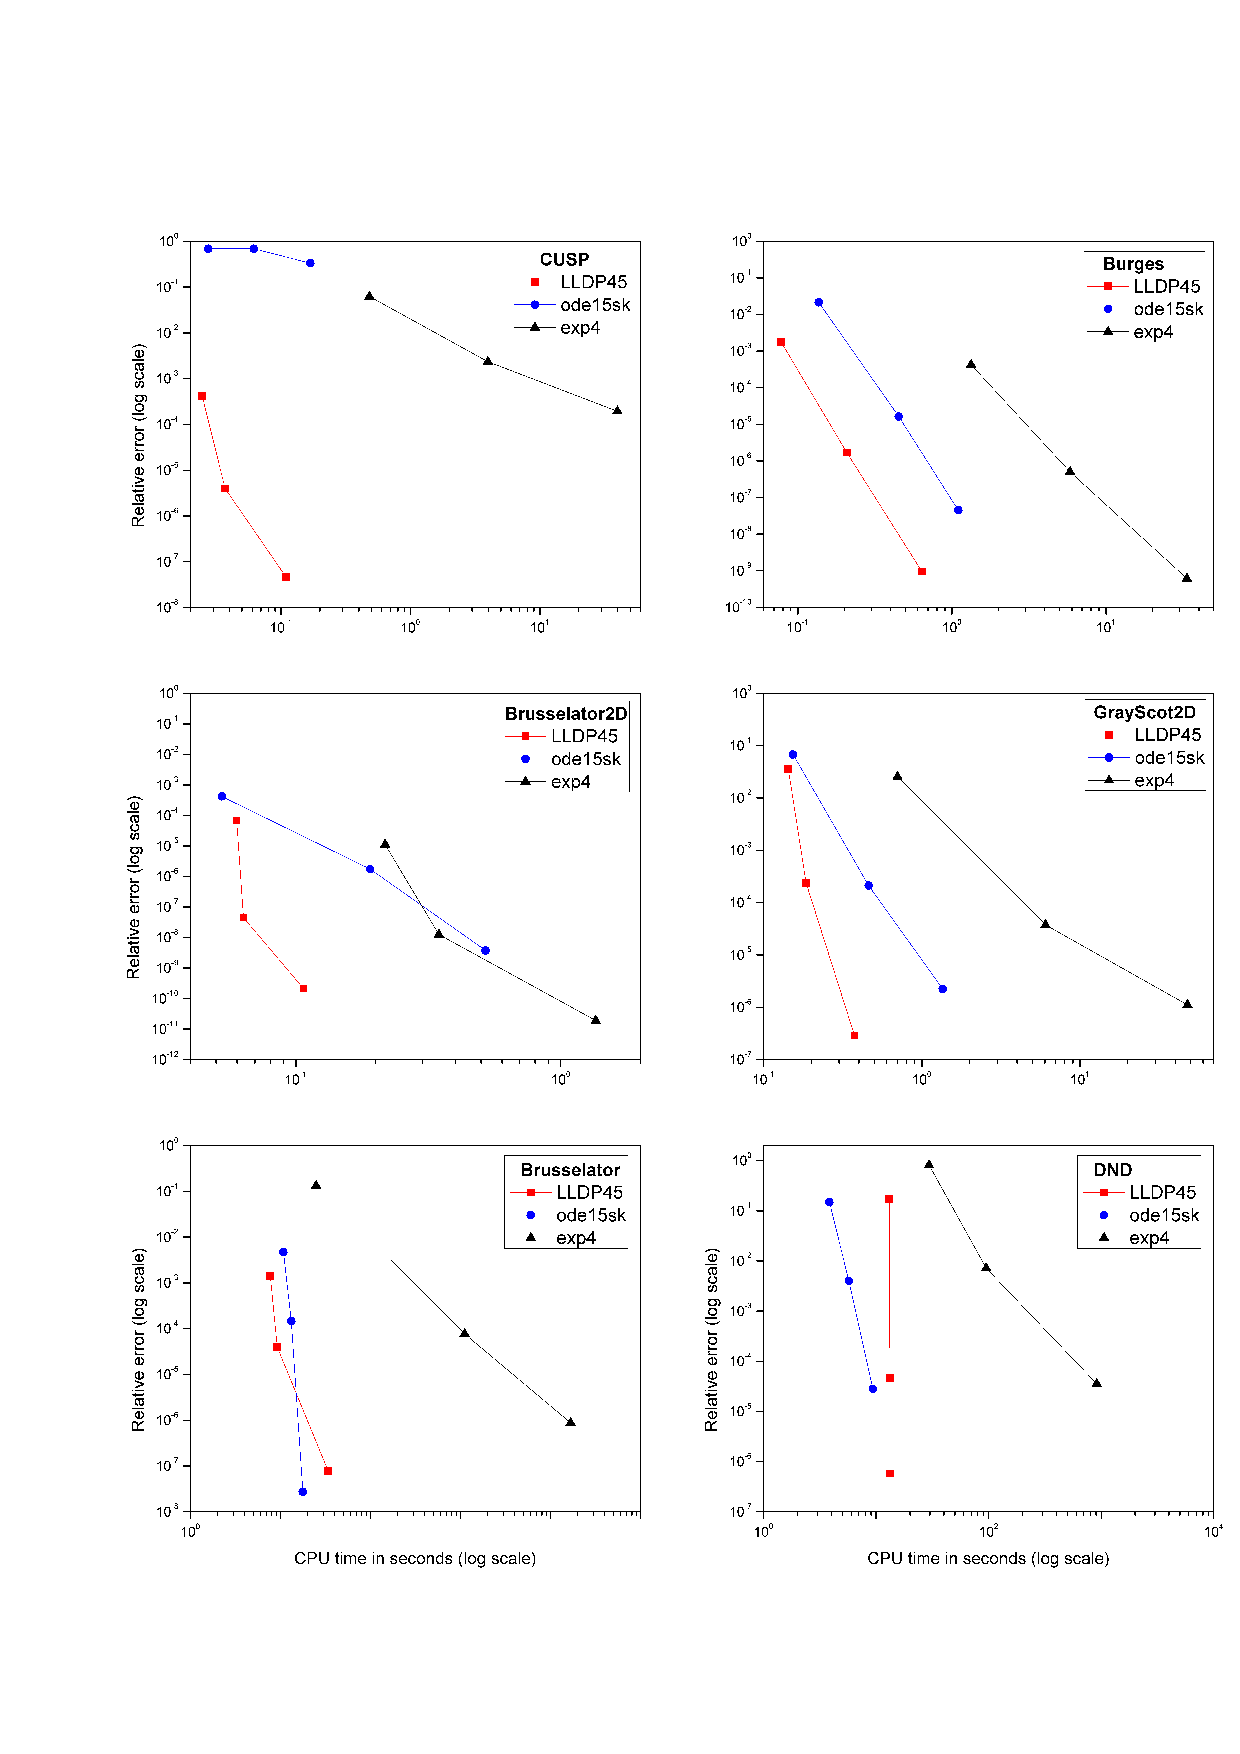
\includegraphics[scale=0.7]{Graphics/lldp-fj/compare_graph.pdf}
		\vspace{-0.95in}
		\caption{Diagrama log-log comparativo de precisión frente a tiempo para cada uno de los códigos en la integración de las seis ecuaciones de prueba. $\vartriangle$: código \emph{JF-ode15sk1}, $\circ$ : código \emph{JF-ode15sk2}, y $\square$: código \emph{JF-LLDP45}}
		\label{lldpfj:Fig1}
	\end{center}
\end{figure}

\begin{table}
	\caption{Desempeño de los códigos \emph{ODE15sk}, \emph{LLDP1}, \emph{LLDP2} y \emph{Exp4} en la integración de las ecuaciones  CUSP y Burgers.}
	\label{tab:cuspburg}
	\begin{adjustbox}{width=0.95\columnwidth,center}
		\begin{tabular}{ccccccccccc}
			\hline
			&  & \multicolumn{4}{c}{CUSP $M=500$, $d=1500$} &  & \multicolumn{4}{c}{Burgers $M=500$, $d=500$} \\
			\cline{3-6}\cline{8-11} & Tol & \emph{ode15sk} & \emph{LLDP1} & \emph{LLDP2} & \emph{exp4jf} &  & \emph{ode15sk} & \emph{LLDP1} & \emph{LLDP2} & \emph{exp4jf} \\
			\hline
			& crude & 1.0000 & 1.6084 & 1.0350 & 1.3776 &  & 1.0000 & 0.5475 & 0.3986 & 1.3144 \\
			RTime & mild & 1.0000 & 0.6442 & 0.4093 & 1.6814 &  & 1.0000 & 0.8583 & 0.5459 & 2.9958 \\
			& refine & 1.0000 & 0.5288 & 0.3385 & 2.7640 &  & 1.0000 & 0.9860 & 0.6277 & 5.3592 \\
			\hline
			& crude & 6.89e-01 & 2.62e-05 & 2.62e-05 & 4.40e-03 &  & 2.06e-02 & 1.72e-03 & 1.70e-03 & 6.30e-03 \\
			RError & mild & 6.88e-01 & 2.49e-06 & 2.49e-06 & 6.64e-04 &  & 1.62e-05 & 1.48e-06 & 1.47e-06 & 1.14e-05 \\
			& refine & 3.32e-01 & 1.28e-08 & 1.81e-08 & 1.65e-07 &  & 4.51e-08 & 4.71e-10 & 6.10e-10 & 1.17e-08 \\
			\hline
			& crude & 24 & 15 & 15 & 11 &  & 244 & 72 & 72 & 80 \\
			A-Steps & mild & 71 & 16 & 16 & 35 &  & 811 & 269 & 269 & 446 \\
			& refine & 188 & 46 & 46 & 178 &  & 2592 & 1068 & 1068 & 2478 \\
			\hline
			& crude & 0 & 0 & 0 & 1 &  & 10 & 3 & 3 & 1 \\
			R-Steps & mild & 3 & 0 & 0 & 0 &  & 10 & 0 & 0 & 1 \\
			& refine & 5 & 1 & 1 & 0 &  & 11 & 0 & 0 & 1 \\
			\hline
			& crude & 180 & 391 & 241 & 128 &  & 2932 & 2189 & 1541 & 1430 \\
			$f$-Eval & mild & 552 & 477 & 287 & 475 &  & 6760 & 8637 & 5158 & 7624 \\
			& refine & 1797 & 1429 & 858 & 2566 &  & 23179 & 34243 & 20326 & 42188 \\
			\hline
			& crude & 24 & 15 & 15 & 36 &  & 254 & 75 & 75 & 243 \\
			K-subspace & mild & 74 & 16 & 16 & 105 &  & 821 & 269 & 269 & 1341 \\
			& refine & 193 & 47 & 47 & 534 &  & 2603 & 1068 & 1068 & 7437 \\
			\hline
			& crude & 36 & 0 & 0 & 0 &  & 492 & 0 & 0 & 0 \\
			LS & mild & 99 & 0 & 0 & 0 &  & 942 & 0 & 0 & 0 \\
			& refine & 281 & 0 & 0 & 0 &  & 2794 & 0 & 0 & 0 \\
			\hline
			& crude & 0 & 15 & 15 & 68 &  & 0 & 146 & 146 & 913 \\
			ME & mild & 0 & 26 & 26 & 292 &  & 0 & 538 & 538 & 4931 \\
			& refine & 0 & 81 & 83 & 1623 &  & 0 & 2135 & 2135 & 27297 \\
			\hline
			& crude & 83 & 60 & 60 & 64 &  & 1703 & 617 & 618 & 1010 \\
			$\mf_{total}$ & mild & 282 & 84 & 84 & 299 &  & 4064 & 1660 & 1660 & 5378 \\
			& refine & 1044 & 262 & 262 & 1675 &  & 14498 & 6442 & 6442 & 29785 \\
			\hline
			& crude & 1 & 4 & 4 & 2 &  & 2 & 4 & 4 & 2 \\
			$\mf_{min}$ & mild & 2 & 4 & 4 & 2 &  & 2 & 4 & 4 & 2 \\
			& refine & 2 & 4 & 4 & 1 &  & 2 & 4 & 4 & 2 \\
			\hline
			& crude & 3 & 4 & 4 & 4 &  & 12 & 31 & 31 & 20 \\
			$\mf_{max}$ & mild & 4 & 6 & 6 & 6 &  & 7 & 12 & 12 & 8 \\
			& refine & 5 & 8 & 8 & 6 &  & 11 & 8 & 8 & 8 \\
			\hline
			& crude & 0 & 3 & 3 & 0 &  & 0 & 3 & 3 & 0 \\
			$\mathfrak{p}_{min}$ & mild & 0 & 3 & 3 & 0 &  & 0 & 3 & 3 & 0 \\
			& refine & 0 & 3 & 3 & 0 &  & 0 & 3 & 3 & 0 \\
			\hline
			& crude & 0 & 3 & 3 & 0 &  & 0 & 3 & 3 & 0 \\
			$\mathfrak{p}_{max}$ & mild & 0 & 3 & 3 & 0 &  & 0 & 3 & 3 & 0 \\
			& refine & 0 & 3 & 3 & 0 &  & 0 & 3 & 3 & 0 \\
			\hline
		\end{tabular}
	\end{adjustbox}
\end{table}

\begin{table}
	\caption{Desempeño de los códigos \emph{ODE15sk}, \emph{LLDP1}, \emph{LLDP2} y \emph{Exp4} en la integración de las ecuaciones the Brusselator2D y GrayScott2D.}
	\label{tab:bruss2DGrayScott}
	\begin{adjustbox}{width=0.95\columnwidth,center}
		\begin{tabular}{ccccccccccc}
			\hline
			&  & \multicolumn{4}{c}{Brusselator2D $M=50$, $d=5000$} &  & \multicolumn{4}{c}{GrayScott2D $M=70$, $d=5000$} \\
			\cline{3-6}\cline{8-11} & Tol & \emph{ode15sk} & \emph{LLDP1} & \emph{LLDP2} & \emph{exp4jf} &  & \emph{ode15sk} & \emph{LLDP1} & \emph{LLDP2} & \emph{exp4jf} \\
			\hline
			& crude & 1.0000 & 1.1690 & 0.9272 & 0.3404 &  & 1.0000 & 0.9495 & 0.6856 & 0.5341 \\
			RTime & mild & 1.0000 & 0.4831 & 0.3717 & 0.3943 &  & 1.0000 & 0.6382 & 0.4613 & 0.7660 \\
			& refine & 1.0000 & 0.0968 & 0.0694 & 0.1913 &  & 1.0000 & 0.1509 & 0.1062 & 0.2434 \\
			\hline
			& crude & 4.17e-04 & 7.16e-06 & 7.16e-06 & 3.79e-04 &  & 7.46e-02 & 2.55e-02 & 2.57e-02 & 2.70e-01 \\
			RError & mild & 1.73e-06 & 2.69e-08 & 2.64e-08 & 1.20e-06 &  & 2.17e-04 & 4.41e-04 & 4.41e-04 & 2.06e-03 \\
			& refine & 3.74e-09 & 1.65e-09 & 1.40e-09 & 1.02e-09 &  & 1.05e-06 & 1.60e-07 & 6.29e-07 & 1.79e-06 \\
			\hline
			& crude & 20 & 13 & 13 & 3 &  & 51 & 16 & 16 & 11 \\
			A-Steps & mild & 59 & 14 & 14 & 7 &  & 133 & 32 & 34 & 20 \\
			& refine & 141 & 23 & 23 & 35 &  & 353 & 104 & 107 & 76 \\
			\hline
			& crude & 0 & 0 & 0 & 0 &  & 0 & 0 & 0 & 0 \\
			R-Steps & mild & 0 & 0 & 0 & 0 &  & 0 & 0 & 0 & 0 \\
			& refine & 0 & 0 & 0 & 1 &  & 3 & 0 & 0 & 2 \\
			\hline
			& crude & 166 & 295 & 212 & 44 &  & 470 & 661 & 409 & 193 \\
			$f$-Eval & mild & 505 & 387 & 261 & 152 &  & 1319 & 1337 & 811 & 737 \\
			& refine & 4362 & 712 & 442 & 694 &  & 12428 & 3527 & 2121 & 2543 \\
			\hline
			& crude & 20 & 13 & 13 & 9 &  & 51 & 16 & 16 & 33 \\
			K-subspace & mild & 59 & 14 & 14 & 21 &  & 133 & 32 & 34 & 60 \\
			& refine & 141 & 23 & 23 & 108 &  & 356 & 104 & 107 & 234 \\
			\hline
			& crude & 26 & 0 & 0 & 0 &  & 63 & 0 & 0 & 0 \\
			LS & mild & 71 & 0 & 0 & 0 &  & 160 & 0 & 0 & 0 \\
			& refine & 281 & 0 & 0 & 0 &  & 694 & 0 & 0 & 0 \\
			\hline
			& crude & 0 & 14 & 14 & 24 &  & 0 & 29 & 30 & 94 \\
			ME & mild & 0 & 25 & 25 & 95 &  & 0 & 64 & 66 & 391 \\
			& refine & 0 & 42 & 42 & 456 &  & 0 & 203 & 210 & 1438 \\
			\hline
			& crude & 93 & 54 & 54 & 28 &  & 292 & 203 & 202 & 137 \\
			$\mf_{total}$ & mild & 303 & 81 & 81 & 116 &  & 865 & 348 & 370 & 636 \\
			& refine & 1752 & 147 & 146 & 506 &  & 5138 & 728 & 733 & 2135 \\
			\hline
			& crude & 2 & 4 & 4 & 1 &  & 2 & 4 & 4 & 1 \\
			$\mf_{min}$ & mild & 2 & 4 & 4 & 2 &  & 2 & 4 & 4 & 2 \\
			& refine & 2 & 4 & 4 & 2 &  & 2 & 4 & 4 & 3 \\
			\hline
			& crude & 6 & 6 & 6 & 8 &  & 13 & 20 & 19 & 15 \\
			$\mf_{max}$ & mild & 7 & 8 & 8 & 11 &  & 15 & 15 & 15 & 20 \\
			& refine & 10 & 8 & 7 & 8 &  & 16 & 8 & 7 & 20 \\
			\hline
			& crude & 0 & 3 & 3 & 0 &  & 0 & 3 & 3 & 0 \\
			$\mathfrak{p}_{min}$ & mild & 0 & 3 & 3 & 0 &  & 0 & 3 & 3 & 0 \\
			& refine & 0 & 3 & 3 & 0 &  & 0 & 3 & 3 & 0 \\
			\hline
			& crude & 0 & 3 & 3 & 0 &  & 0 & 3 & 3 & 0 \\
			$\mathfrak{p}_{max}$ & mild & 0 & 3 & 3 & 0 &  & 0 & 3 & 3 & 0 \\
			& refine & 0 & 3 & 3 & 0 &  & 0 & 3 & 3 & 0 \\
			\hline
		\end{tabular}
	\end{adjustbox}
\end{table}

\begin{table}
	\caption{Desempeño de los códigos \emph{ODE15sk}, \emph{LLDP1}, \emph{LLDP2} y \emph{Exp4} en la integración de las ecuaciones Brusselator y DND.}
	\label{tab:brussdnd}
	\begin{adjustbox}{width=0.95\columnwidth,center}
		\begin{tabular}{ccccccccccc}
			\hline
			&  & \multicolumn{4}{c}{Brusselator $M=500$, $d=1000$} &  & \multicolumn{4}{c}{DND $M=500$, $d=500$} \\
			\cline{3-6}\cline{8-11} & Tol & \emph{ode15sk} & \emph{LLDP1} & \emph{LLDP2} & \emph{exp4jf} &  & \emph{ode15sk} & \emph{LLDP1} & \emph{LLDP2} & \emph{exp4jf} \\
			\hline
			& crude & 1.0000 & 7.4488 & 4.7279 & 2.4839 &  & 1.0000 & 1.2543 & 0.8419 & 1.5636 \\
			RTime & mild & 1.0000 & 6.5767 & 4.1338 & 2.3521 &  & 1.0000 & 0.7711 & 0.5240 & 1.9486 \\
			& refine & 1.0000 & 6.3426 & 3.9840 & 4.2940 &  & 1.0000 & 0.2582 & 0.1764 & 1.4330 \\
			\hline
			& crude & 8.83e-04 & 5.42e-04 & 3.38e-04 & 1.65e-03 &  & 1.58e-03 & 8.36e-04 & 8.36e-04 & 8.89e-03 \\
			RError & mild & 1.99e-05 & 6.83e-07 & 8.23e-07 & 2.86e-06 &  & 2.14e-06 & 8.24e-07 & 9.19e-07 & 3.17e-06 \\
			& refine & 2.06e-07 & 1.12e-09 & 1.12e-09 & 9.37e-10 &  & 4.55e-09 & 8.98e-10 & 8.91e-10 & 3.82e-09 \\
			\hline
			& crude & 31 & 367 & 368 & 54 &  & 51 & 94 & 94 & 10 \\
			A-Steps & mild & 85 & 821 & 821 & 104 &  & 167 & 97 & 97 & 47 \\
			& refine & 219 & 2577 & 2578 & 315 &  & 453 & 201 & 203 & 253 \\
			\hline
			& crude & 0 & 0 & 1 & 0 &  & 0 & 1 & 1 & 1 \\
			R-Steps & mild & 0 & 0 & 0 & 0 &  & 0 & 2 & 2 & 3 \\
			& refine & 0 & 0 & 0 & 0 &  & 0 & 1 & 1 & 3 \\
			\hline
			& crude & 1059 & 15487 & 8886 & 1394 &  & 999 & 3119 & 1844 & 411 \\
			$f$-Eval & mild & 2320 & 31025 & 17973 & 2900 &  & 2235 & 3885 & 2238 & 1370 \\
			& refine & 6755 & 87521 & 51503 & 15214 &  & 10175 & 7131 & 4212 & 5490 \\
			\hline
			& crude & 31 & 367 & 369 & 162 &  & 51 & 95 & 95 & 33 \\
			K-subspace & mild & 85 & 821 & 821 & 312 &  & 167 & 99 & 99 & 150 \\
			& refine & 219 & 2577 & 2578 & 945 &  & 453 & 202 & 204 & 768 \\
			\hline
			& crude & 50 & 0 & 0 & 0 &  & 78 & 0 & 0 & 0 \\
			LS & mild & 114 & 0 & 0 & 0 &  & 194 & 0 & 0 & 0 \\
			& refine & 306 & 0 & 0 & 0 &  & 530 & 0 & 0 & 0 \\
			\hline
			& crude & 0 & 693 & 709 & 568 &  & 0 & 189 & 188 & 187 \\
			ME & mild & 0 & 1620 & 1617 & 1338 &  & 0 & 198 & 196 & 806 \\
			& refine & 0 & 5152 & 5154 & 7303 &  & 0 & 402 & 405 & 3586 \\
			\hline
			& crude & 927 & 4114 & 4127 & 1123 &  & 791 & 617 & 617 & 320 \\
			$\mf_{total}$ & mild & 2006 & 7324 & 7324 & 2379 &  & 1678 & 972 & 971 & 1093 \\
			& refine & 5432 & 17992 & 17990 & 13638 &  & 4814 & 1552 & 1567 & 4183 \\
			\hline
			& crude & 5 & 4 & 4 & 6 &  & 3 & 5 & 5 & 2 \\
			$\mf_{min}$ & mild & 4 & 4 & 4 & 2 &  & 3 & 7 & 7 & 2 \\
			& refine & 3 & 4 & 4 & 2 &  & 3 & 6 & 6 & 2 \\
			\hline
			& crude & 20 & 14 & 15 & 27 &  & 16 & 11 & 11 & 27 \\
			$\mf_{max}$ & mild & 20 & 11 & 11 & 27 &  & 15 & 15 & 15 & 20 \\
			& refine & 20 & 8 & 8 & 20 &  & 14 & 8 & 8 & 15 \\
			\hline
			& crude & 0 & 3 & 3 & 0 &  & 0 & 3 & 3 & 0 \\
			$\mathfrak{p}_{min}$ & mild & 0 & 3 & 3 & 0 &  & 0 & 3 & 3 & 0 \\
			& refine & 0 & 3 & 3 & 0 &  & 0 & 3 & 3 & 0 \\
			\hline
			& crude & 0 & 3 & 3 & 0 &  & 0 & 3 & 3 & 0 \\
			$\mathfrak{p}_{max}$ & mild & 0 & 3 & 3 & 0 &  & 0 & 3 & 3 & 0 \\
			& refine & 0 & 3 & 3 & 0 &  & 0 & 3 & 3 & 0 \\
			\hline
		\end{tabular}
	\end{adjustbox}
\end{table}

\begin{table}
	\caption{Valores mínimos y máximos de $\alpha _{1}$ y $\alpha _{2}$ correspondientes a los valores de estos parámetros en el esquema \emph{LLDP1} al integrar las seis ecuaciones de prueba. $r^{min}-r^{max}$ es el rango de fluctuaciones en la velocidad de convergencia $r$ del integrador \emph{LLDP1} durante el proceso de integración. Los símbolos $+$ y $*$ indican, respectivamente, intercambios de fórmulas de diferencias finitas dentro del algoritmo \ref{alg:iArnoldi} o en la expresión (\ref{Jacobian-free LLDPK scheme}) durante el proceso de integración.}
	\label{tab:R_LLDP1}
	\begin{adjustbox}{width=0.95\columnwidth,center}
		\begin{tabular}{lccccccccccc}
			& \multicolumn{3}{c}{$\alpha^{min}_{1}-\alpha^{max}_{1}$} &  & \multicolumn{3}{c}{$\alpha^{min}_{2}-\alpha^{max}_{2}$} &  & \multicolumn{3}{c}{$r^{min}-r^{max}$} \\
			\cline{2-4}\cline{6-8}\cline{10-12} Example & Crude & Mild & Refine &  & Crude & Mild & Refine &  & Crude & Mild & Refine \\
			\hline
			CUSP & \multicolumn{1}{l}{0.9-1.4} & \multicolumn{1}{l}{0.8-1.4} & \multicolumn{1}{l}{0.8-1.3} &  & \multicolumn{1}{l}{0.6-1.5} & \multicolumn{1}{l}{0.5-1.5} & \multicolumn{1}{l}{0.4-1.3} &  & \multicolumn{1}{l}{2-3} & \multicolumn{1}{l}{2-3} & \multicolumn{1}{l}{2-3} \\
			Burgers & \multicolumn{1}{l}{3.1-5.6$^+$} & \multicolumn{1}{l}{2.2-4.1$^+$} & \multicolumn{1}{l}{2.0-3.1} &  & \multicolumn{1}{l}{2.7-5.8*} & \multicolumn{1}{l}{1.7-3.9*} & \multicolumn{1}{l}{1.4-2.7} &  & \multicolumn{1}{l}{5-5} & \multicolumn{1}{l}{5-5} & \multicolumn{1}{l}{5-5} \\
			Brusselator2D & \multicolumn{1}{l}{1.6-3.4} & \multicolumn{1}{l}{1.4-3.4} & \multicolumn{1}{l}{1.3-3.2} &  & \multicolumn{1}{l}{1.2-3.4*} & \multicolumn{1}{l}{0.9-3.4*} & \multicolumn{1}{l}{0.7-3.2*} &  & \multicolumn{1}{l}{4-5} & \multicolumn{1}{l}{3-5} & \multicolumn{1}{l}{3-5} \\
			GrayScott2D & \multicolumn{1}{l}{1.4-3.5} & \multicolumn{1}{l}{1.2-3.0} & \multicolumn{1}{l}{1.1-2.4} &  & \multicolumn{1}{l}{0.9-3.7*} & \multicolumn{1}{l}{0.7-2.8} & \multicolumn{1}{l}{0.6-2.2} &  & \multicolumn{1}{l}{3-5} & \multicolumn{1}{l}{3-5} & \multicolumn{1}{l}{3-5} \\
			Brusselator & \multicolumn{1}{l}{1.7-2.8} & \multicolumn{1}{l}{1.5-2.4} & \multicolumn{1}{l}{1.3-2.1} &  & \multicolumn{1}{l}{1.2-2.5} & \multicolumn{1}{l}{0.9-2.0} & \multicolumn{1}{l}{0.7-1.5} &  & \multicolumn{1}{l}{4-5} & \multicolumn{1}{l}{4-5} & \multicolumn{1}{l}{3-5} \\
			DND & \multicolumn{1}{l}{2.1-2.5} & \multicolumn{1}{l}{1.9-2.5} & \multicolumn{1}{l}{1.6-2.3} &  & \multicolumn{1}{l}{1.6-2.1} & \multicolumn{1}{l}{1.4-2.1} & \multicolumn{1}{l}{1.1-1.7} &  & \multicolumn{1}{l}{5-5} & \multicolumn{1}{l}{4-5} & \multicolumn{1}{l}{4-5} \\
			\hline
		\end{tabular}
	\end{adjustbox}
\end{table}

.


\begin{table}
	\caption{Valores mínimos y máximos de $\alpha _{1}$ y $\alpha _{2}$ correspondientes a los valores de estos parámetros en el esquema \emph{LLDP2} al integrar las seis ecuaciones de prueba. $r^{min}-r^{max}$ es el rango de fluctuaciones en la velocidad de convergencia $r$ del integrador \emph{LLDP2} durante el proceso de integración. Los símbolos $+$ y $*$ indican, respectivamente, intercambios de fórmulas de diferencias finitas dentro del algoritmo \ref{alg:iArnoldi} o en la expresión (\ref{Jacobian-free LLDPK scheme}) durante el proceso de integración.}
	\label{tab:R_LLDP2}
	\begin{adjustbox}{width=0.95\columnwidth,center}
		\begin{tabular}{lccccccccccc}
			& \multicolumn{3}{c}{$\alpha^{min}_{1}-\alpha^{max}_{1}$} &  & \multicolumn{3}{c}{$\alpha^{min}_{2}-\alpha^{max}_{2}$} &  & \multicolumn{3}{c}{$r^{min}-r^{max}$} \\
			\cline{2-4}\cline{6-8}\cline{10-12} Example & Crude & Mild & Refine &  & Crude & Mild & Refine &  & Crude & Mild & Refine \\
			\hline
			CUSP & \multicolumn{1}{l}{0.9-1.4} & \multicolumn{1}{l}{0.8-1.4} & \multicolumn{1}{l}{0.8-1.3} &  & \multicolumn{1}{l}{0.6-1.5} & \multicolumn{1}{l}{0.5-1.5} & \multicolumn{1}{l}{0.4-1.3} &  & \multicolumn{1}{l}{1-2} & \multicolumn{1}{l}{1-2} & \multicolumn{1}{l}{1-2} \\
			Burgers & \multicolumn{1}{l}{3.1-5.6} & \multicolumn{1}{l}{2.2-4.1} & \multicolumn{1}{l}{2.0-3.1} &  & \multicolumn{1}{l}{2.7-5.8*} & \multicolumn{1}{l}{1.7-3.9*} & \multicolumn{1}{l}{1.4-2.7} &  & \multicolumn{1}{l}{4-5} & \multicolumn{1}{l}{3-5} & \multicolumn{1}{l}{3-4} \\
			Brusselator2D & \multicolumn{1}{l}{1.6-3.4} & \multicolumn{1}{l}{1.4-3.4} & \multicolumn{1}{l}{1.3-3.2} &  & \multicolumn{1}{l}{1.2-3.4*} & \multicolumn{1}{l}{0.9-3.4*} & \multicolumn{1}{l}{0.7-3.2*} &  & \multicolumn{1}{l}{2-4} & \multicolumn{1}{l}{2-4} & \multicolumn{1}{l}{2-4} \\
			GrayScott2D & \multicolumn{1}{l}{1.4-3.5} & \multicolumn{1}{l}{1.2-3.0} & \multicolumn{1}{l}{1.1-2.4} &  & \multicolumn{1}{l}{0.9-3.7*} & \multicolumn{1}{l}{0.7-2.8} & \multicolumn{1}{l}{0.6-2.1} &  & \multicolumn{1}{l}{2-4} & \multicolumn{1}{l}{2-3} & \multicolumn{1}{l}{2-3} \\
			Brusselator & \multicolumn{1}{l}{1.7-2.8} & \multicolumn{1}{l}{1.5-2.4} & \multicolumn{1}{l}{1.3-2.1} &  & \multicolumn{1}{l}{1.2-2.5} & \multicolumn{1}{l}{0.9-2.0} & \multicolumn{1}{l}{0.7-1.5} &  & \multicolumn{1}{l}{2-3} & \multicolumn{1}{l}{2-3} & \multicolumn{1}{l}{2-3} \\
			DND & \multicolumn{1}{l}{2.1-2.5} & \multicolumn{1}{l}{1.9-2.5} & \multicolumn{1}{l}{1.6-2.3} &  & \multicolumn{1}{l}{1.6-2.1} & \multicolumn{1}{l}{1.5-2.1} & \multicolumn{1}{l}{1.1-1.7} &  & \multicolumn{1}{l}{3-3} & \multicolumn{1}{l}{2-3} & \multicolumn{1}{l}{2-3} \\
			\hline
		\end{tabular}
	\end{adjustbox}
\end{table}